%% ===========================================================================
%%  Manuscript for Urban Climate (Elsevier)  ---  elsarticle, review format
%%  Compile with:  tectonic -X compile manuscript.tex
%%
%%  STATUS: Methods section complete and grounded in the actual pipeline.
%%          Title / Abstract / Introduction / Results / Discussion / Conclusion
%%          are [PLACEHOLDER] stubs for the co-authors to complete.
%%          Citation keys are placeholders: each \bibitem states the INTENDED
%%          source (marked "verify") or [PLACEHOLDER] where a domain reference
%%          is still needed. No reference has been asserted as final.
%% ===========================================================================
\documentclass[review,11pt]{elsarticle}

\usepackage{lineno}
\usepackage{amsmath,amssymb}
\usepackage{graphicx}
\usepackage{booktabs}
\usepackage{array}
\usepackage{url}

\graphicspath{{../outputs/figures/}}

\newcommand{\degC}{\ensuremath{^{\circ}\mathrm{C}}}
\newcommand{\ph}[1]{\textbf{[PLACEHOLDER: #1]}}
\newcommand{\vi}{\textbf{[verify-intended]}}

\journal{Urban Climate}

\begin{document}

\begin{frontmatter}

%% ---- Title -------------------------------------------------------------
\title{Where and How Fast Is Heat Stress Worsening? A District-Level, Multi-Index
Machine-Learning Projection for 64 districts of Bangladesh }

%% ---- Authors (5 entries; author~1 is complete, 2--5 are copies to rename)
\author[bup]{Mohammad Khalid Hasan Nabil\corref{cor1}}
\ead{nabil23549009015@student.bup.edu.bd}

\author[bup]{Mohammad} % [PLACEHOLDER: co-author 2 name]
\author[bup]{Khalid} % [PLACEHOLDER: co-author 3 name]
\author[bup]{Hasan Nabil} % [PLACEHOLDER: co-author 4 name]
\author[bup]{Nabil} % [PLACEHOLDER: co-author 5 name]

\affiliation[bup]{organization={Department of Information Communication Technology,
    Faculty of Science and Technology, Bangladesh University of Professionals},
    city={Dhaka},
    postcode={1216},
    country={Bangladesh}}

\cortext[cor1]{Corresponding author. ORCID: 0009-0007-3255-1420}

%% ---- Abstract ----------------------------------------------------------
\begin{abstract}
Rising heat and humidity increasingly threaten health, labour, and energy systems
across Bangladesh, yet operational planning needs district-resolved,
uncertainty-aware projections of the specific conditions that drive human heat
stress. We present a deterministic, reproducible machine-learning framework that
projects seven temperature-correlated heat-stress conditions---heat-index comfort,
wet-bulb temperature, indoor and outdoor wet-bulb globe temperature, cooling
degree-days, ultraviolet exposure, and dew-point moisture stress---for all 64
districts of Bangladesh. Four gradient-boosting ensembles are trained on the
2014--2024 monthly record using future-known seasonal features; the observed
1980--2024 Theil--Sen trend is superimposed so that projections evolve
realistically, and all thermal indices are recomputed from the projected primary
variables to avoid target leakage. Validated against withheld 2025 observations,
the projected indices attain median $R^{2}$ of $0.95$--$0.98$, and their
operational risk classes match observations to within one class in $100\%$ of
district-months. A Mann--Kendall analysis shows maximum temperature rising in
every district (median $+0.56\,^{\circ}$C per decade) while minimum temperature
remains flat, indicating a widening diurnal range; the coastal and southwestern
zones carry the greatest combined burden, and ultraviolet and oppressive-humidity
hazards are effectively nationwide. District choropleths, zonal envelopes, and
calibrated uncertainty bands provide a directly actionable heat-stress outlook
while transparently bounding the models' skill relative to climatology.
\end{abstract}

%% ---- Keywords (suggested; editable) ------------------------------------
\begin{keyword}
heat stress \sep wet-bulb temperature \sep WBGT \sep seasonal projection \sep
gradient boosting \sep Mann--Kendall trend \sep Bangladesh \sep climate adaptation
\end{keyword}

\end{frontmatter}

\linenumbers

%% ===========================================================================
\section{Introduction}\label{sec:intro}
Anthropogenic climate change has fundamentally altered the frequency, intensity,
and duration of extreme heat events worldwide. Mean surface air temperatures have
risen steadily since the pre-industrial era, and this warming has been accompanied
by a disproportionate increase in heatwaves, prolonged humid spells, and compound
heat--humidity extremes that the human body increasingly struggles to tolerate
\citep{Shaw2022IPCCAsia}. Unlike many climate hazards, extreme heat acts as a
silent stressor, producing cumulative physiological strain that is frequently
underreported in official mortality and morbidity statistics yet carries
substantial public-health, occupational, and economic consequences
\citep{Kjellstrom2019}. Understanding how heat stress manifests across different
climatic and geographic settings has therefore become an urgent priority for
adaptation planning.

Air temperature alone does not represent the heat stress the human body actually
experiences and can lead to misleading assessments. Relative humidity, solar
radiation, wind, and atmospheric moisture all govern the body's ability to shed
heat through evaporation, radiation, and convection; elevated humidity in
particular suppresses the evaporation of sweat---the body's primary cooling
mechanism---so that core temperature rises even when the air is not exceptionally
hot \citep{steadman1979}. To capture these combined effects, researchers have
developed composite heat-stress indices that now underpin public-health warning
systems, occupational heat-safety standards \citep{iso7243_2017}, and cooling-energy
demand projections \citep{spinoni2018}, and that increasingly recognise the
approach of physiological survivability limits under extreme humid heat
\citep{raymond2020}.

South Asia is among the regions most acutely exposed to escalating heat stress,
owing to its dense population, high monsoon-season humidity, and large share of
outdoor and informal-sector labour. Bangladesh occupies a uniquely exposed
position within it: a tropical monsoon climate, low-lying deltaic geography, and
exceptionally high population density combine with rapid, unplanned urbanization
to let heat stress intensify quickly and distribute unevenly across the landscape
\citep{Sultana2021}. Critically, the country is not climatically homogeneous---its
territory spans drought-prone northwestern plains with continental microclimates,
a densely built and heat-retentive central urban core exhibiting strong urban
heat-island effects, low-lying coastal districts shaped by maritime humidity,
seasonally inundated wetland basins, and elevated hill tracts with distinct
topographic regimes. Each zone is expected to experience thermal stress through
different pathways and at different intensities, yet most existing heat-risk
assessments in Bangladesh continue to treat the country as a single climatic unit
or rely on a narrow selection of indices---most commonly ambient temperature
alone---without accounting for the multi-dimensional nature of heat exposure
\citep{Abrar2022}.

A parallel gap exists in temporal scope and forecasting capability. Most prior
work on heat stress in Bangladesh is retrospective in orientation or resolved only
to divisional or national summaries, and very few studies integrate long-term
climatological baselines with near-term machine-learning forecasting to project
how thermal stress will evolve at the district level~\vi. This omission matters,
because heat-risk management---whether through early-warning systems, occupational
health policy, or urban cooling infrastructure---requires knowing not only where
risk is highest today but where and how quickly it is worsening. A recent
wet-bulb globe temperature analysis across Bangladesh reported warming of roughly
0.08--0.5\,\degC per decade, most pronounced in the southeast and northeast
\citep{kamal2024scientific}, underscoring the need for district-resolved, multi-index
projection.

This study addresses these gaps through the Temperature-Correlated Conditions
(TCC) framework: an integrated set of seven temperature-dependent indicators
---heat-index comfort, wet-bulb temperature, indoor and outdoor wet-bulb globe
temperature, heatstroke risk, cooling degree-days, ultraviolet exposure, and
dew-point moisture stress---each capturing a distinct physiological, biophysical,
or infrastructural dimension of heat-related risk. Applying this framework to
45~years (1980--2024) of district-level meteorological records across all
64~districts and six climatically distinct zones, we (i)~train an ensemble of
gradient-boosting models \citep{Breiman2001} on future-known seasonal features and
re-impose the observed long-term trend so that projections evolve realistically
rather than collapsing onto the last training year; (ii)~recompute every thermal
index from the projected primary variables rather than predicting the indices
directly, eliminating target leakage and preserving the physical coupling among
temperature, humidity, and radiation; (iii)~generate 24-month district-level
projections (2025--2026) with analytically propagated uncertainty bands; and
(iv)~validate the projections out-of-sample against independent 2025 observations,
benchmark their skill transparently against seasonal-naive and climatological
baselines, and characterise long-term change with the non-parametric
Mann--Kendall test. The best model per variable is selected by a multi-attribute
simple-additive-weighting scheme with a generalization-gap penalty
\citep{Hwang1981}.

Two features distinguish the analysis. First, results are reported at full
district resolution through choropleth maps rather than aggregated away, exposing
spatial gradients---such as the coastal concentration of humid-heat burden---that
zonal summaries obscure. Second, we are explicit about the limits of predictive
skill: at monthly resolution the ensembles essentially match climatology, so their
value lies in providing spatially complete, uncertainty-aware, and
trend-consistent projections of physiologically relevant indices rather than in
reducing monthly error. One indicator, heatstroke risk, was found to lack
out-of-sample skill and is retained only descriptively. The remainder of this
paper details the data and methods, presents the validated projections and
observed trends, and discusses their implications for heat-adaptation planning
across Bangladesh.

%% ===========================================================================
\section{Literature Review}\label{sec:litreview}

Human exposure to heat is not adequately captured by dry-bulb air temperature
alone. A growing body of work therefore evaluates compound thermal indices that
combine temperature with humidity, radiation, and wind to describe how heat is
actually experienced and how it threatens health, labour productivity, and energy
demand. This section synthesises recent international and Bangladesh-focused
literature across the seven temperature-correlated conditions addressed in this
study, the machine-learning methods used to forecast them, and the urban and
regional context that motivates a district-resolved, multi-index treatment.

\subsection{The physiological basis of thermal-stress indices}
\citet{raymond2020} provided seminal evidence that a wet-bulb temperature (WBT)
of $35\,\degC$ represents the physiological limit for human survival, showing that
humid-heat extremes had already more than doubled in frequency between 1979 and
2017 and shifting the field's focus from ambient temperature toward compound
heat--humidity metrics. The inadequacy of dry-bulb temperature as a standalone
indicator is well established: high humidity impairs the evaporative efficiency of
perspiration, causing perceived loads to exceed measured air temperature
\citep{steadman1979}. The heat index formalises this through the regression of
\citet{rothfusz1990}, operationalised by the U.S.\ National Weather Service. The
wet-bulb globe temperature (WBGT), originally developed by \citet{yaglou1957} for
military training and codified in ISO~7243 \citep{iso7243_2017}, extends the
framework to radiant load, making it the international standard for occupational
heat-stress assessment \citep{parsons2006}. The empirical WBT approximation of
\citet{stull2011}, derived by gene-expression programming with a mean absolute
error below $0.3\,\degC$, provides a computationally efficient estimate applicable
to station and reanalysis data alike. Cooling degree-days (CDD) complement these
physiological indices by quantifying the cumulative thermal energy above a
baseline, a standard proxy for building cooling demand \citep{spinoni2018,
bhatnagar2018}; the UV index \citep{who2002} captures the solar-radiation
dimension of outdoor exposure; and dew-point temperature offers a stable,
temperature-independent measure of atmospheric moisture that outperforms relative
humidity as a predictor of perceived discomfort \citep{lawrence2005}. Together
these conditions span the physiological, biophysical, and infrastructural
dimensions of heat risk that the present study projects jointly, against a
backdrop of accelerating global warming documented by the IPCC \citep{ipcc2022ar6}.

\subsection{Observed heat-stress trends in Bangladesh}
Bangladesh is among the most heat-exposed nations, and a dense body of
station-based work documents its warming. \citet{rahman2021} produced the first
comprehensive spatiotemporal appraisal of historical and projected heat-index
change, finding statistically significant upward trends across most districts,
sharpest in the pre-monsoon season. \citet{tanim2024heat} analysed 60~years
(1961--2020) of records from 17 stations using the Discomfort Index, Humidex, and
WBT, reporting a spatially uneven rise in heat discomfort that is steepest along
the coastal belt and driven primarily by rising air temperature. For WBGT
specifically, \citet{kamal2024scientific} provided the anchor analysis, computing
outdoor WBGT from 1979--2021 reanalysis with the physically based Liljegren model
and finding a national rise of $0.08$--$0.5\,\degC$ per decade, a fivefold
expansion of the area affected by high-to-extreme stress, and air temperature as
the dominant driver ($85.9\%$ relative importance); a companion paper developed
simplified regression equations to lower the computational barrier to WBGT
adoption \citep{kamal2024ijc}. Temperature-extreme indices are likewise
intensifying: \citet{ahmed2022} found lengthening warm-spell durations,
particularly in coastal regions, and \citet{islam2021extremes} identified
warm-index trends dominated by post-2000 increases across 27 stations. Trends in
degree-days were examined by \citet{islam2020cdd}, who reported significant CDD
increases with the southwestern and central zones showing the highest annual
means. At the health end, \citet{miah2026} linked ambient temperature and heat
index to heatstroke mortality in an ecological time-series analysis, reinforcing
the public-health urgency of a multi-index approach.

\subsection{Urban heat islands and zone-specific dynamics}
Urban heat-island (UHI) intensity amplifies background warming, especially within
the densely built central zone examined here. \citet{dewan2021} characterised
diurnal and seasonal UHI across five major Bangladeshi cities from satellite
land-surface temperature, finding the greatest magnitude in the pre-monsoon period
and the largest daytime surface UHI in Dhaka ($2.74\,\degC$), followed by
Chittagong ($1.92\,\degC$) and Khulna ($1.27\,\degC$). \citet{faisal2022} reported
that UHI intensity rose substantially across most districts from 2000 to 2020,
with Dhaka and Mymensingh steepest, and \citet{park2024} showed that Dhaka's UHI
is strongest in winter ($0.95\,\degC$) and weakest during the monsoon
($0.23\,\degC$), with heat waves producing distinctive synoptic patterns that
compound local warming. These findings support treating Bangladesh's urban core as
a distinct climatic zone and, more broadly, motivate the six-zone structure adopted
in this study.

\subsection{Machine learning for meteorological and thermal-index forecasting}
Ensemble tree methods have consistently outperformed conventional statistical and
numerical approaches for temperature and humidity forecasting in data-rich,
strongly seasonal settings. The gradient-boosting family---XGBoost
\citep{chen2016xgboost}, LightGBM \citep{ke2017lightgbm}, and CatBoost
\citep{prokhorenkova2018catboost}---recurs as a strong, interpretable baseline
across environmental prediction problems. In Bangladesh, \citet{islam2026enso}
found XGBoost most accurate for seasonal temperature prediction across 29 stations
($R^{2}=0.88$ for maximum and $0.97$ for minimum temperature) when trained on ENSO
predictors; \citet{akter2025} found Random Forest best for humidity forecasting at
northern stations over a 40-year record; and \citet{rahman2024rnlstm} found a
stacking ensemble outperformed RNN--LSTM and decision-forest models for
average-temperature prediction over a 60-year series. Most directly,
\citet{mollah2026mlheatindex} benchmarked ARIMAX, SARIMAX, Random Forest, XGBoost,
and LSTM on 3-hourly Dhaka records (2014--2023) for conditional, scenario-based
heat-index projection, with Random Forest achieving the lowest error
(RMSE~$=0.85\,\degC$, $R^{2}=0.987$)---a close methodological precedent for the
present work. The value of combining gradient-boosting learners is illustrated by
\citet{kim2023toxins}, whose stacked XGBoost/LightGBM/CatBoost ensemble reached
$R^{2}=0.93$, outperforming any single model. Fourier-based encoding of seasonal
cycles as sine and cosine terms has been shown to improve both accuracy and
efficiency on meteorological series \citep{galansales2024}, directly motivating the
Fourier feature layer used here. Comparative studies elsewhere reinforce the
transferability of these methods \citep{hanoon2021ml,abdelsattar2025ml}, while the
validation of deep-learning weather models on recent extreme events
\citep{pasche2025validating} and analyses of the distinct atmospheric drivers of
humidex versus temperature heatwaves \citep{jeong2025humidex} situate the
forecasting problem in its broader physical context.

\subsection{Per-condition modelling and international context}
Beyond the anchor WBGT and heat-index studies, the individual conditions have
distinct literatures. For the heat-index/Humidex family, \citet{sojan2024humidheat}
showed that humid-heat stress in India is intensifying disproportionately faster
than dry heat; \citet{kushwaha2026humidex} projected air temperature as the
dominant driver of future extreme-Humidex days across 15 CMIP6 models;
\citet{scoccimarro2017humidity} established that perceived-temperature extremes
intensify faster than temperature extremes owing to rising humidity;
\citet{saha2025postescalation} documented a post-2000 escalation of humid heatwaves
across Northeast India and Bangladesh; and \citet{tabassum2025coolroofs} connected
a cool-roof intervention to measurable Humidex reductions during a Dhaka heat wave.
Heatstroke-risk modelling has matured chiefly outside Bangladesh---%
\citet{xuh2024heatstroke} trained interpretable models linking meteorology to
heatstroke incidence in South China---with \citet{ehsan2026extremeheat} providing a
recent Bangladesh-focused machine-learning forecast of extreme-heat health impact;
consistent with this thin evidence base, the present study computes a heatstroke
indicator but, as reported below, excludes it from the validated results for a lack
of out-of-sample skill. For CDD, \citet{bilgili2023cdd} showed that classical
SARIMA models remain competitive with machine learning when the seasonal structure
is strong. UV-index modelling is comparatively underexplored in the regional
literature: \citet{teggi2026uvindex} recently derived the UV index from reanalysis
validated against ground stations, whereas in the present framework the UV index is
instead predicted directly as a modelled variable. Dew-point prediction has a
well-developed machine-learning lineage, progressing from extreme-learning-machine
and kernel baselines \citep{mohammadi2015elm,qasem2019dewpoint}, to gradient-boosted
trees exploiting cross-station information \citep{yao2022catboost}, to
attention-based sequence models with explainability \citep{abdullah2025xai}.
Internationally, the stakes are large: \citet{parsons2021labor} estimated humid-heat
labour losses equivalent to roughly $1.7\%$ of 2017 global GDP, with South Asian
outdoor workers among the worst affected, and \citet{flouris2022} meta-analysed a
significant negative association between WBGT exposure and manual work capacity.
Longer-term projections for Bangladesh under CMIP6 \citep{khatun2024} indicate
continued rises in warm-spell duration and tropical nights, providing the
multi-decadal backdrop against which the near-term (2025--2026) forecasts generated
here should be read.

\subsection{Research gaps addressed by this study}
Three gaps emerge from this review. First, although individual indices---chiefly
WBGT and the heat index---have been examined for Bangladesh in isolation, no study
has simultaneously computed, validated, and forecast seven complementary
thermal-stress conditions within a single framework, at district resolution, across
climatically distinct zones. Second, existing Bangladeshi forecasting work has
relied on conventional statistics, CMIP6 downscaling, or single-algorithm machine
learning; the multi-algorithm gradient-boosting ensemble with Fourier feature
engineering and an explicitly re-imposed observational trend proposed here has not
previously been applied to thermal-stress forecasting in this context. Third, the
six-zone climatological structure of Bangladesh---Northwest dry-hot plains, Central
urban core, Southwest saline-drought belt, Coastal maritime zone, Haor wetland
basins, and Hill Tracts---has not previously organised a multi-index heat-risk
assessment, leaving intra-national thermal heterogeneity systematically
undercharacterised. In contrast to studies built on ERA5 reanalysis, the present
work is driven by station-derived Visual Crossing records and validated
out-of-sample against independent 2025 observations, providing an externally
verified, uncertainty-aware, and district-resolved projection across all seven
conditions.

%% ===========================================================================
\section{Materials and Methods}\label{sec:methods}

This study builds a deterministic, reproducible pipeline that (i) learns the
monthly climatology of seven primary meteorological variables for each of the
64 districts of Bangladesh from a recent, high-quality window; (ii) superimposes
the long-term observed climate trend so that projections evolve realistically
beyond the training period; (iii) recomputes physiologically relevant thermal
indices from the projected primary variables to avoid target leakage; (iv)
quantifies projection uncertainty by first-order error propagation; and (v)
validates the projected 2025 fields against independent observations. All
methodological constants are fixed a~priori and are reported here so that the
workflow can be audited and reproduced exactly.

\subsection{Study area and climatic zonation}\label{sec:zones}
The analysis covers all 64 administrative districts of Bangladesh. For synthesis
and reporting, districts are grouped into six climatic zones: (1)~Northwest
Extreme Heat Zone (dry hot plains, including the Barind Tract), (2)~Central Urban
Heat Zone (urban heat-island region), (3)~Southwest Hot--Dry Zone (drought- and
salinity-affected areas), (4)~Coastal Humid Heat Zone (the coastal belt),
(5)~Haor/Wetland Humid Zone (the haor basin), and (6)~Hill Tract Zone (elevated
terrain). The zonation is author-defined but grounded in converging, established
frameworks: the agro-climatic regionalisation of the Bangladesh Meteorological
Department and the agro-ecological/physiographic zonation of Bangladesh
\citep{FAO1988,Rashid1991}, together with recognised hydro-ecological units
(Barind Tract, Sundarbans coastal belt, haor basin). Each district is flagged as
a \emph{confirmed} (high-confidence) or \emph{provisional} assignment, and one
representative \emph{exemplar} district per zone is retained for main-text
figures (Figure~\ref{fig:mapzones}). The complete district-to-zone mapping is
provided in the supplementary material.

\begin{figure}[htbp]
\centering
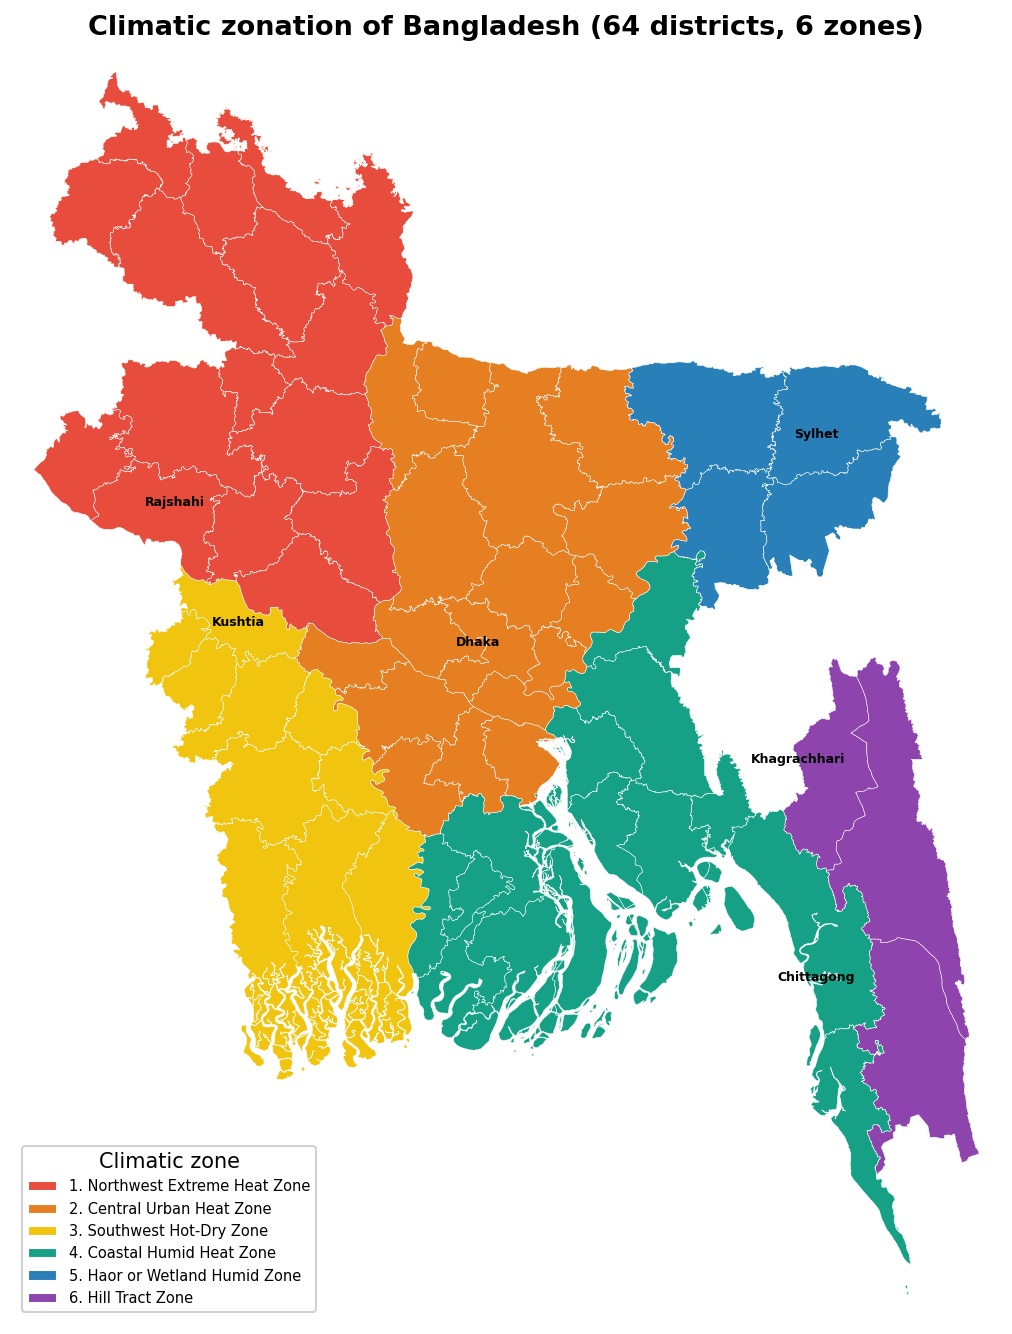
\includegraphics[width=0.72\linewidth]{map_zonation.png}
\caption{Climatic zonation of Bangladesh: the 64 districts grouped into six
zones, with the exemplar district of each zone labelled.}
\label{fig:mapzones}
\end{figure}

\subsection{Data and preprocessing}\label{sec:data}
Daily meteorological records were obtained from the Visual Crossing Weather API
\citep{vc} for each district. Seven primary (physically measured)
variables are used: mean, maximum, and minimum near-surface air temperature
($\degC$); relative humidity (\%); dew-point temperature ($\degC$); downward
solar (shortwave) radiation; and the ultraviolet (UV) index. The historical
record spans 1980--2024; an additional file covering 2025 (through 20~November
2025; the final month is partial) is reserved exclusively for out-of-sample
validation.

Because humidity is noisy in the earliest decades and solar/UV are unavailable
before 2014, the machine-learning window is restricted to
2014--2024, whereas the full 1980--2024 record is used only for the
observational trend analysis (Section~\ref{sec:trend}). Daily values are
aggregated to calendar-month means (month-start resampling), and residual gaps
are filled by linear interpolation. All modelling is performed on these monthly
series.

\subsection{Feature construction}\label{sec:features}
To respect a strict \emph{future-known-features-only} constraint---no lags,
rolling windows, or autoregressive terms that would be unavailable at projection
time---each month is described by a deterministic seasonal--secular feature
vector. Seasonality is encoded by a truncated Fourier series with period
$P=12$~months and $H=3$ harmonics,
\begin{equation}
\sin_{h}(m)=\sin\!\Big(\tfrac{2\pi h m}{P}\Big),\qquad
\cos_{h}(m)=\cos\!\Big(\tfrac{2\pi h m}{P}\Big),\qquad h=1,\dots,H,
\end{equation}
where $m$ is the calendar-month index. The secular component is the calendar
year. The full design vector is therefore
$\mathbf{x}=[\,\mathrm{year},\ \sin_{1},\cos_{1},\dots,\sin_{3},\cos_{3}\,]$
(seven features).

\subsection{Predictive models}\label{sec:models}
Four gradient-based tree ensembles are trained independently for every
district--variable pair: Random Forest \citep{Breiman2001}, XGBoost
\citep{chen2016xgboost}, LightGBM \citep{ke2017lightgbm}, and CatBoost
\citep{prokhorenkova2018catboost}. Hyperparameters are fixed a~priori and applied
uniformly across all districts and variables so that results are mutually
comparable and the pipeline is fully deterministic (global random seed $=42$).
The fixed configurations are listed in the supplementary material.

\subsection{Trend-aware detrending and projection}\label{sec:detrend}
Tree ensembles cannot extrapolate beyond the range of their training features;
if the calendar year is used directly as a predictor, every projected year
collapses onto the last training year, producing a static (trendless) forecast.
To carry the observed climate trend forward while preserving the future-known
constraint, each primary variable is detrended before learning and re-trended at
prediction time. For district--variable series $y(t)$ with continuous time $t$
(in years), a Theil--Sen slope $\hat{\beta}$ is estimated from the
annual-mean series,
\begin{equation}
\hat{\beta}=\operatorname{median}_{\,i<j}
\frac{\bar{y}_{j}-\bar{y}_{i}}{t_{j}-t_{i}},
\label{eq:theilsen}
\end{equation}
where $\bar{y}_{k}$ is the mean of year $k$. To keep the projected trend
consistent with the manuscript's observational trend analysis, $\hat{\beta}$ is
taken from the robust 1980--2024 record for the five variables that span it
(mean/max/min temperature, humidity, dew point); solar radiation and the UV
index, which lack a pre-2014 record, fall back to a Theil--Sen fit over their
available 2014--2024 window. The ensembles are trained on the deseasonalised
residual $r(t)=y(t)-\hat{\beta}\,t$, so they model only the seasonal signal;
the linear trend is added back at prediction time,
$\hat{y}(t)=\hat{r}(t)+\hat{\beta}\,t$. This design makes each projected year
differ from the previous one by exactly $\hat{\beta}$ and guarantees that the
projected inter-annual tendency equals the reported Mann--Kendall/Sen slope
(Section~\ref{sec:trend}). We emphasise that this trend term is included for
physical consistency with the observed record, not to improve short-horizon
accuracy: at monthly resolution the seasonal cycle dominates, so the trend
contributes only a small secular adjustment.

The winning model per variable (Section~\ref{sec:saw}) is refit on the full
2014--2024 residual and projected forward for a 24-month horizon (January~2025
through December~2026). Projected primary variables are clipped to
physically plausible bounds before any downstream computation to prevent
non-physical extrapolations from propagating into the indices.

\subsection{Model evaluation and selection}\label{sec:saw}
Reported test metrics use a strictly chronological hold-out: models are trained
on 2014--2022 and tested on the withheld 2023--2024 period. Generalisation is
additionally assessed by five-fold \texttt{TimeSeriesSplit} cross-validation on
the residual series. For each candidate model we record the coefficient of
determination $R^{2}$ and root-mean-square error (RMSE) on the chronological
test set, the cross-validated $R^{2}$ ($\mathrm{CV}\text{-}R^{2}$), a
generalisation gap $\mathrm{Gap}=\lvert R^{2}-\mathrm{CV}\text{-}R^{2}\rvert$,
and an operational tolerance accuracy $A_{\tau}$ defined as the fraction of test
months whose absolute error does not exceed a variable-specific tolerance
$\tau$,
\begin{equation}
A_{\tau}=\frac{1}{N}\sum_{n=1}^{N}\mathbf{1}\!\big(\lvert y_{n}-\hat{y}_{n}\rvert
\le \tau\big).
\end{equation}

The winning model is chosen by Simple Additive Weighting (SAW), a multi-attribute
decision-making scheme \citep{Hwang1981}, with a generalisation-gap penalty. Each criterion $c$ is min--max normalised across the
four candidates---directly for benefit criteria and by complement for cost
criteria,
\begin{equation}
\tilde{s}_{c}=
\begin{cases}
\dfrac{s_{c}-\min_{c}}{\max_{c}-\min_{c}}, & c\ \text{maximised},\\[1.2ex]
\dfrac{\max_{c}-s_{c}}{\max_{c}-\min_{c}}, & c\ \text{minimised},
\end{cases}
\end{equation}
and the composite score is the weighted sum
$S=\sum_{c} w_{c}\,\tilde{s}_{c}$, with weights $w_{R^{2}}=0.25$,
$w_{\mathrm{CV}\text{-}R^{2}}=0.25$, $w_{\mathrm{RMSE}}=0.20$,
$w_{\mathrm{Gap}}=0.20$, and $w_{A_{\tau}}=0.10$ (RMSE and Gap treated as cost
criteria). The highest-scoring model wins; models with $\mathrm{Gap}>0.10$ are
additionally flagged as overfitting risks.

\subsection{Thermal index computation}\label{sec:indices}
To avoid target leakage, thermal-stress indices are never predicted directly;
they are recomputed analytically from the \emph{projected} primary variables.
The heat index (HI) uses the U.S.\ National Weather Service Rothfusz regression
\citep{rothfusz1990}. With temperature $T_F$ and relative humidity $R$ (in
$^{\circ}$F and \%),
\begin{align}
\mathrm{HI} =\ & -42.379 + 2.04901523\,T_F + 10.14333127\,R
     - 0.22475541\,T_F R \nonumber\\
   & - 6.83783\!\times\!10^{-3} T_F^{2}
     - 5.481717\!\times\!10^{-2} R^{2}
     + 1.22874\!\times\!10^{-3} T_F^{2} R \nonumber\\
   & + 8.5282\!\times\!10^{-4} T_F R^{2}
     - 1.99\!\times\!10^{-6} T_F^{2} R^{2},
\label{eq:hi}
\end{align}
with the standard low-humidity and high-humidity adjustments applied within
their validity ranges and a simplified formula substituted below $80^{\circ}$F;
the result is returned in $\degC$. Wet-bulb temperature $T_w$ follows the
empirical formulation of \citet{stull2011},
\begin{align}
T_w =\ & T\,\arctan\!\big[0.151977\,(R+8.313659)^{1/2}\big]
       + \arctan(T+R) \nonumber\\
     & - \arctan(R-1.676331)
       + 0.00391838\,R^{3/2}\arctan(0.023101\,R) - 4.686035,
\label{eq:wetbulb}
\end{align}
with $T$ in $\degC$ and $R$ in \%. Wet-bulb globe temperature is computed in a
shade variant (no direct-beam term) and a sun variant that adds a
solar-radiation contribution $S$,
\begin{align}
\mathrm{WBGT}_{\text{shade}} &= 0.7\,T_w + 0.3\,T, \label{eq:wbgtshade}\\
\mathrm{WBGT}_{\text{sun}}   &= 0.7\,T_w + 0.2\,(T + 0.025\,S) + 0.1\,T.
\label{eq:wbgtsun}
\end{align}
Cooling degree-days are expressed as a monthly-mean daily rate about an
$18\,\degC$ base,
\begin{equation}
\mathrm{CDD}=\max\!\Big(\tfrac{T_{\max}+T_{\min}}{2}-18,\ 0\Big).
\label{eq:cdd}
\end{equation}

A composite heatstroke-hazard score (a sigmoid of the heat index modulated by a
wet-bulb multiplier) was also implemented and recalibrated for monthly-mean
inputs. However, in external validation it produced a negative out-of-sample
$R^{2}$ (i.e.\ worse than a constant predictor), so it is \emph{excluded from all
predictive results} and retained only as a descriptive projected field. This
exclusion is stated explicitly to avoid over-interpretation of an index that
does not demonstrate skill.

\subsection{Operational heat-stress conditions and risk categorisation}
\label{sec:conditions}
The projected fields are organised into seven temperature-correlated heat-stress
conditions of operational relevance: (1)~heat-index comfort (perceived
temperature under humidity); (2)~wet-bulb temperature (the thermodynamic limit of
evaporative cooling); (3)~wet-bulb globe temperature in indoor (shade) and outdoor
(sun) forms (the occupational heat-exposure standard); (4)~heatstroke risk;
(5)~cooling degree-days (a building-cooling energy proxy); (6)~ultraviolet
exposure risk; and (7)~dew-point moisture stress. Conditions~(6) and~(7) are
obtained directly from the projected UV-index and dew-point fields, which are
among the primary modelled variables (Section~\ref{sec:data}); condition~(4) is
excluded from predictive results as noted above.

To move from continuous values to operational meaning, four of the conditions are
additionally mapped to established risk-category systems: the U.S.\ National
Weather Service heat-index comfort classes (Comfortable, Caution, Extreme
Caution, Danger, Extreme Danger); WBGT occupational-exposure classes (Low,
Moderate, High, Extreme); the World Health Organization UV-index classes (Low,
Moderate, High, Very High, Extreme) \citep{who2002}; and dew-point human-comfort
classes (Dry through Extremely Oppressive). Wet-bulb temperature~(2) and cooling
degree-days~(5) are reported as continuous physical quantities. The category
boundaries are conventionally defined for daily peak values; because the present
pipeline operates on monthly means, the extreme classes are seldom reached and
the categories should be read as describing \emph{typical monthly} conditions
rather than daily peaks. Categorisation skill is assessed against the observed
2025 fields by exact-match agreement and by agreement to within one adjacent
class.

\subsection{Uncertainty quantification}\label{sec:uncertainty}
Projection uncertainty for the temperature--humidity indices is obtained by
first-order (linearised) error propagation from the primary-variable
uncertainties. For an index $I(x_1,\dots,x_k)$ with input standard deviations
$\sigma_{x_j}$,
\begin{equation}
\sigma_{I}=\Bigg[\sum_{j}\Big(\tfrac{\partial I}{\partial x_j}\Big)^{2}
\sigma_{x_j}^{2}\Bigg]^{1/2},
\label{eq:errprop}
\end{equation}
where the input $\sigma_{x_j}$ are taken from each winning model's in-sample
RMSE and representative sensitivity coefficients are used for the heat index,
wet-bulb temperature, and WBGT. The propagated $\sigma_{I}$ define the
$68\%$ ($\pm\sigma_{I}$) and $95\%$ ($\pm1.96\,\sigma_{I}$) bands reported for
the projected indices.

\subsection{Baseline skill benchmarks}\label{sec:baselines}
Model skill is benchmarked against two references evaluated on the same
chronological test set: a seasonal-naive predictor (each test month set to the
same calendar month one year earlier) and a monthly-climatology predictor (the
training-period mean for each calendar month). Skill relative to a reference is
\begin{equation}
\mathrm{SS}=1-\frac{\mathrm{RMSE}_{\text{model}}}{\mathrm{RMSE}_{\text{ref}}},
\label{eq:skill}
\end{equation}
so that positive values indicate improvement over the reference.

\subsection{External validation against observed 2025}\label{sec:validation}
The 24-month projection includes calendar year 2025, for which independent
observations were withheld from all training. Projected monthly primary
variables and recomputed indices are compared with the observed 2025 monthly
series using $R^{2}$, RMSE, mean absolute error, and the tolerance-accuracy
bands of Section~\ref{sec:saw}. The final month (November~2025) is partial in the
source data and is treated accordingly. This constitutes a genuine, fully
out-of-sample test of the projection.

\subsection{Observational trend analysis}\label{sec:trend}
Long-term trends are characterised on the full 1980--2024 annual-mean series
using the non-parametric Mann--Kendall test with Theil--Sen slope estimation,
computed independently of the predictive models (and therefore free of target
leakage). The Mann--Kendall statistic is
\begin{equation}
S=\sum_{k=1}^{n-1}\sum_{j=k+1}^{n}\operatorname{sgn}(x_j-x_k),
\end{equation}
with tie-corrected variance
\begin{equation}
\operatorname{Var}(S)=\frac{n(n-1)(2n+5)-\sum_{i} t_i(t_i-1)(2t_i+5)}{18},
\end{equation}
where $t_i$ is the number of ties of extent $i$. The standardised statistic
\begin{equation}
Z=\begin{cases}
(S-1)/\sqrt{\operatorname{Var}(S)}, & S>0,\\
0, & S=0,\\
(S+1)/\sqrt{\operatorname{Var}(S)}, & S<0,
\end{cases}
\end{equation}
is referred to the standard normal distribution for a two-sided $p$-value, and
Kendall's $\tau=2S/[n(n-1)]$ measures rank correlation with time. The Theil--Sen
slope (Eq.~\ref{eq:theilsen}) provides the trend magnitude, reported per decade.
Trends with $p<0.05$ are deemed significant. This analysis is performed for mean,
maximum, and minimum temperature, humidity, dew point, and the
temperature--humidity indices (heat index, wet-bulb temperature, shade WBGT)
that are computable across the full record.

A subset of districts encode pre-$\sim$2000 missing days as zero in the source
record; left uncorrected, the resulting $0\rightarrow\sim\!30\,\degC$ step
fabricates physically impossible trends (an artefactual $+7.8\,\degC$ per decade
in one district). Before any trend is fit, daily values below physically
plausible floors ($5\,\degC$ for temperatures, with lower floors for minimum
temperature and dew point, and $5\%$ for humidity) are therefore treated as
missing, and a year must retain at least 60 valid days to enter the annual-mean
series. The same masked slopes are used when the trend is re-added to the
projection (Section~\ref{sec:detrend}). This affects only the observational
trend and long-run slope; the machine-learning models are unaffected because they
train exclusively on the complete 2014--2024 window.

\subsection{Zonal synthesis}\label{sec:zonal}
District-level projections are summarised by zone as monthly and annual
envelopes (the minimum, mean, and maximum across member districts) for the key
indices, providing compact, journal-page-efficient views of the projected
heat-stress distribution in place of 64 individual district panels. Full
district-level detail is additionally retained through choropleth maps rendered
directly from the CC BY 3.0 IGO geoBoundaries Bangladesh ADM2 administrative
boundaries \citep{GeoBoundaries2020}; districts are matched to the boundary geometry
by name, and per-district values are mapped for the observed trends, the projected
annual means of all seven conditions, and the number of months per year each
district spends in each condition's hazard class.

\subsection{Implementation and reproducibility}\label{sec:impl}
The pipeline is implemented in Python~3.14 using scikit-learn~1.8
\citep{Pedregosa2011}, LightGBM~4.6, XGBoost~3.3, CatBoost~1.2.10, together with
NumPy, pandas, and Matplotlib. All stochastic components use a fixed seed, and a
run manifest records package versions, configuration constants, and per-run
timings so that every reported artefact is traceable to a specific
configuration.

%% ===========================================================================
\section{Results}\label{sec:results}

The full pipeline was executed for all 64 districts, producing 448
district--variable models, a 24-month projection (January~2025--December~2026)
per district, an out-of-sample validation against observed 2025, and the
1980--2024 observational trend analysis. Unless stated otherwise, statistics are
reported as the median across the 64 districts.

\subsection{Predictive accuracy and model selection}\label{sec:res-models}
On the chronological 2023--2024 hold-out, the ensembles reproduced the primary
variables accurately, with median test $R^{2}$ of 0.970 for minimum temperature,
0.961 for mean temperature, 0.962 for dew point, and 0.886 for maximum
temperature; humidity (0.632), solar radiation (0.691), and the UV index (0.664)
were intrinsically harder and scored lower. Under the SAW criterion, LightGBM was
selected most frequently (284 of 448 fits), followed by Random Forest (111) and
CatBoost (53); XGBoost, although included in the candidate pool, was never
top-ranked. Model preference was variable-dependent (Table~\ref{tab:models}):
LightGBM dominated temperature (57/64), maximum temperature (63/64), and dew
point (48/64), whereas Random Forest was preferred for the noisier humidity
field (55/64) and was competitive for solar radiation and UV.

\begin{table}[htbp]
\centering
\caption{Best-model selection frequency across the 64 districts, by variable
(SAW criterion). XGBoost was never selected and is omitted.}
\label{tab:models}
\begin{tabular}{lccc}
\toprule
Variable & LightGBM & Random Forest & CatBoost \\
\midrule
Mean temperature      & 57 &  0 &  7 \\
Maximum temperature   & 63 &  0 &  1 \\
Minimum temperature   & 44 &  2 & 18 \\
Relative humidity     &  4 & 55 &  5 \\
Dew point             & 48 &  0 & 16 \\
Solar radiation       & 29 & 29 &  6 \\
UV index              & 39 & 25 &  0 \\
\bottomrule
\end{tabular}

\end{table}

\subsection{External validation against observed 2025}\label{sec:res-val}
The projected 2025 fields, produced without any exposure to 2025 observations,
validated strongly (Table~\ref{tab:validation}). Median $R^{2}$ reached 0.982 for
minimum temperature, 0.980 for dew point, and 0.950 for mean temperature (RMSE
$0.72\,\degC$). Crucially, the thermal-stress indices---recomputed from the
projected primary variables rather than predicted directly---also validated well:
wet-bulb temperature and shade WBGT both at $R^{2}=0.969$ (RMSE $\le
0.63\,\degC$), sun WBGT at 0.966, the heat index at 0.951 (RMSE $1.36\,\degC$),
and cooling degree-days at 0.951. Maximum temperature (0.845), humidity (0.825),
UV (0.805), and solar radiation (0.766) were the weakest, consistent with their
lower learnability. For the six exemplar districts, heat-index validation $R^{2}$
ranged from 0.873 (Sylhet) and 0.891 (Chittagong) to 0.948--0.954 (Kushtia,
Khagrachhari, Rajshahi, Dhaka), with RMSE between $1.1$ and $1.9\,\degC$.

\begin{table}[htbp]
\centering
\caption{External validation of the projected 2025 fields against observed 2025,
summarised as the median across 64 districts. Errors are in each variable's
native unit ($\degC$ for temperatures and thermal indices; \% for humidity;
W\,m$^{-2}$ for solar radiation; index units for UV; $\degC$\,d\,d$^{-1}$ for
CDD).}
\label{tab:validation}
\begin{tabular}{lcccc}
\toprule
Variable & $n$ & Median $R^{2}$ & Median RMSE & Median MAE \\
\midrule
Mean temperature    & 64 & 0.950 & 0.720 & 0.615 \\
Maximum temperature & 64 & 0.845 & 0.940 & 0.788 \\
Minimum temperature & 64 & 0.982 & 0.565 & 0.449 \\
Relative humidity   & 64 & 0.825 & 2.334 & 1.996 \\
Dew point           & 64 & 0.980 & 0.601 & 0.469 \\
Solar radiation     & 64 & 0.766 & 14.352 & 11.704 \\
UV index            & 64 & 0.805 & 0.375 & 0.302 \\
\midrule
Heat index          & 64 & 0.951 & 1.357 & 1.142 \\
Wet-bulb temperature & 64 & 0.969 & 0.624 & 0.509 \\
WBGT (shade)        & 64 & 0.969 & 0.595 & 0.506 \\
WBGT (sun)          & 64 & 0.966 & 0.644 & 0.543 \\
Cooling degree-days & 64 & 0.951 & 0.696 & 0.577 \\
\bottomrule
\end{tabular}

\end{table}

\subsection{Skill relative to baselines}\label{sec:res-skill}
Against the seasonal-naive reference the ensembles were skilful in 81.5\% of
district--variable cases, with the largest median gains for minimum temperature
($+0.24$) and dew point ($+0.21$). Relative to monthly climatology, however, the
models were essentially at parity: the median skill score was near zero or
slightly negative for every variable (e.g.\ $-0.003$ for mean temperature,
$-0.030$ for maximum temperature, $-0.059$ for minimum temperature), and only
31.9\% of cases exceeded climatology. This is the expected behaviour at monthly
resolution: the ensembles reconstruct the strong tropical seasonal cycle that
monthly climatology already encodes, so they add little in raw error terms. Their
contribution is therefore not a reduction in monthly RMSE but a spatially
complete, uncertainty-quantified, and trend-consistent projection that
climatology cannot provide.

\subsection{Observed long-term trends, 1980--2024}\label{sec:res-trend}
The Mann--Kendall/Sen analysis revealed a coherent warming signal
(Table~\ref{tab:trends}, Figure~\ref{fig:maptrend}). Maximum temperature
increased significantly in all 64 districts (median $+0.56\,\degC$ per decade),
and the heat index, wet-bulb temperature, and shade WBGT increased in 58, 57, and
58 of 64 districts (median $+0.37$, $+0.17$, and $+0.17\,\degC$ per decade,
respectively). Mean temperature rose in 50 districts and dew point in 46. Minimum
temperature was markedly more heterogeneous (16 increasing, 13 decreasing, 35
without significant trend; median $+0.02\,\degC$ per decade), and humidity was
mixed (24 increasing, 23 decreasing). The sharp contrast between near-universal
maximum-temperature warming and the essentially flat minimum-temperature signal
indicates a widening diurnal temperature range in much of the country; a small
number of districts (e.g.\ Sylhet) therefore show a slight decrease in \emph{mean}
temperature despite rising maxima. Because the projection re-imposes exactly these
Sen slopes, the projected inter-annual tendency reproduces this observed signal by
construction.

\begin{table}[htbp]
\centering
\caption{Observed 1980--2024 trends (Mann--Kendall test with Theil--Sen slope) by
variable: number of districts increasing, decreasing, or without a significant
trend ($p<0.05$), and the median Sen slope per decade ($\degC$ per decade, except
humidity in \% per decade).}
\label{tab:trends}
\begin{tabular}{lcccc}
\toprule
Variable & Increasing & Decreasing & No trend & Median slope/decade \\
\midrule
Maximum temperature   & 64 &  0 &  0 & $+0.558$ \\
Mean temperature      & 50 &  2 & 12 & $+0.194$ \\
Minimum temperature   & 16 & 13 & 35 & $+0.021$ \\
Dew point             & 46 &  0 & 18 & $+0.197$ \\
Relative humidity     & 24 & 23 & 17 & $+0.177$ \\
Heat index            & 58 &  1 &  5 & $+0.373$ \\
Wet-bulb temperature  & 57 &  0 &  7 & $+0.165$ \\
WBGT (shade)          & 58 &  0 &  6 & $+0.172$ \\
\bottomrule
\end{tabular}

\end{table}

\begin{figure}[htbp]
\centering
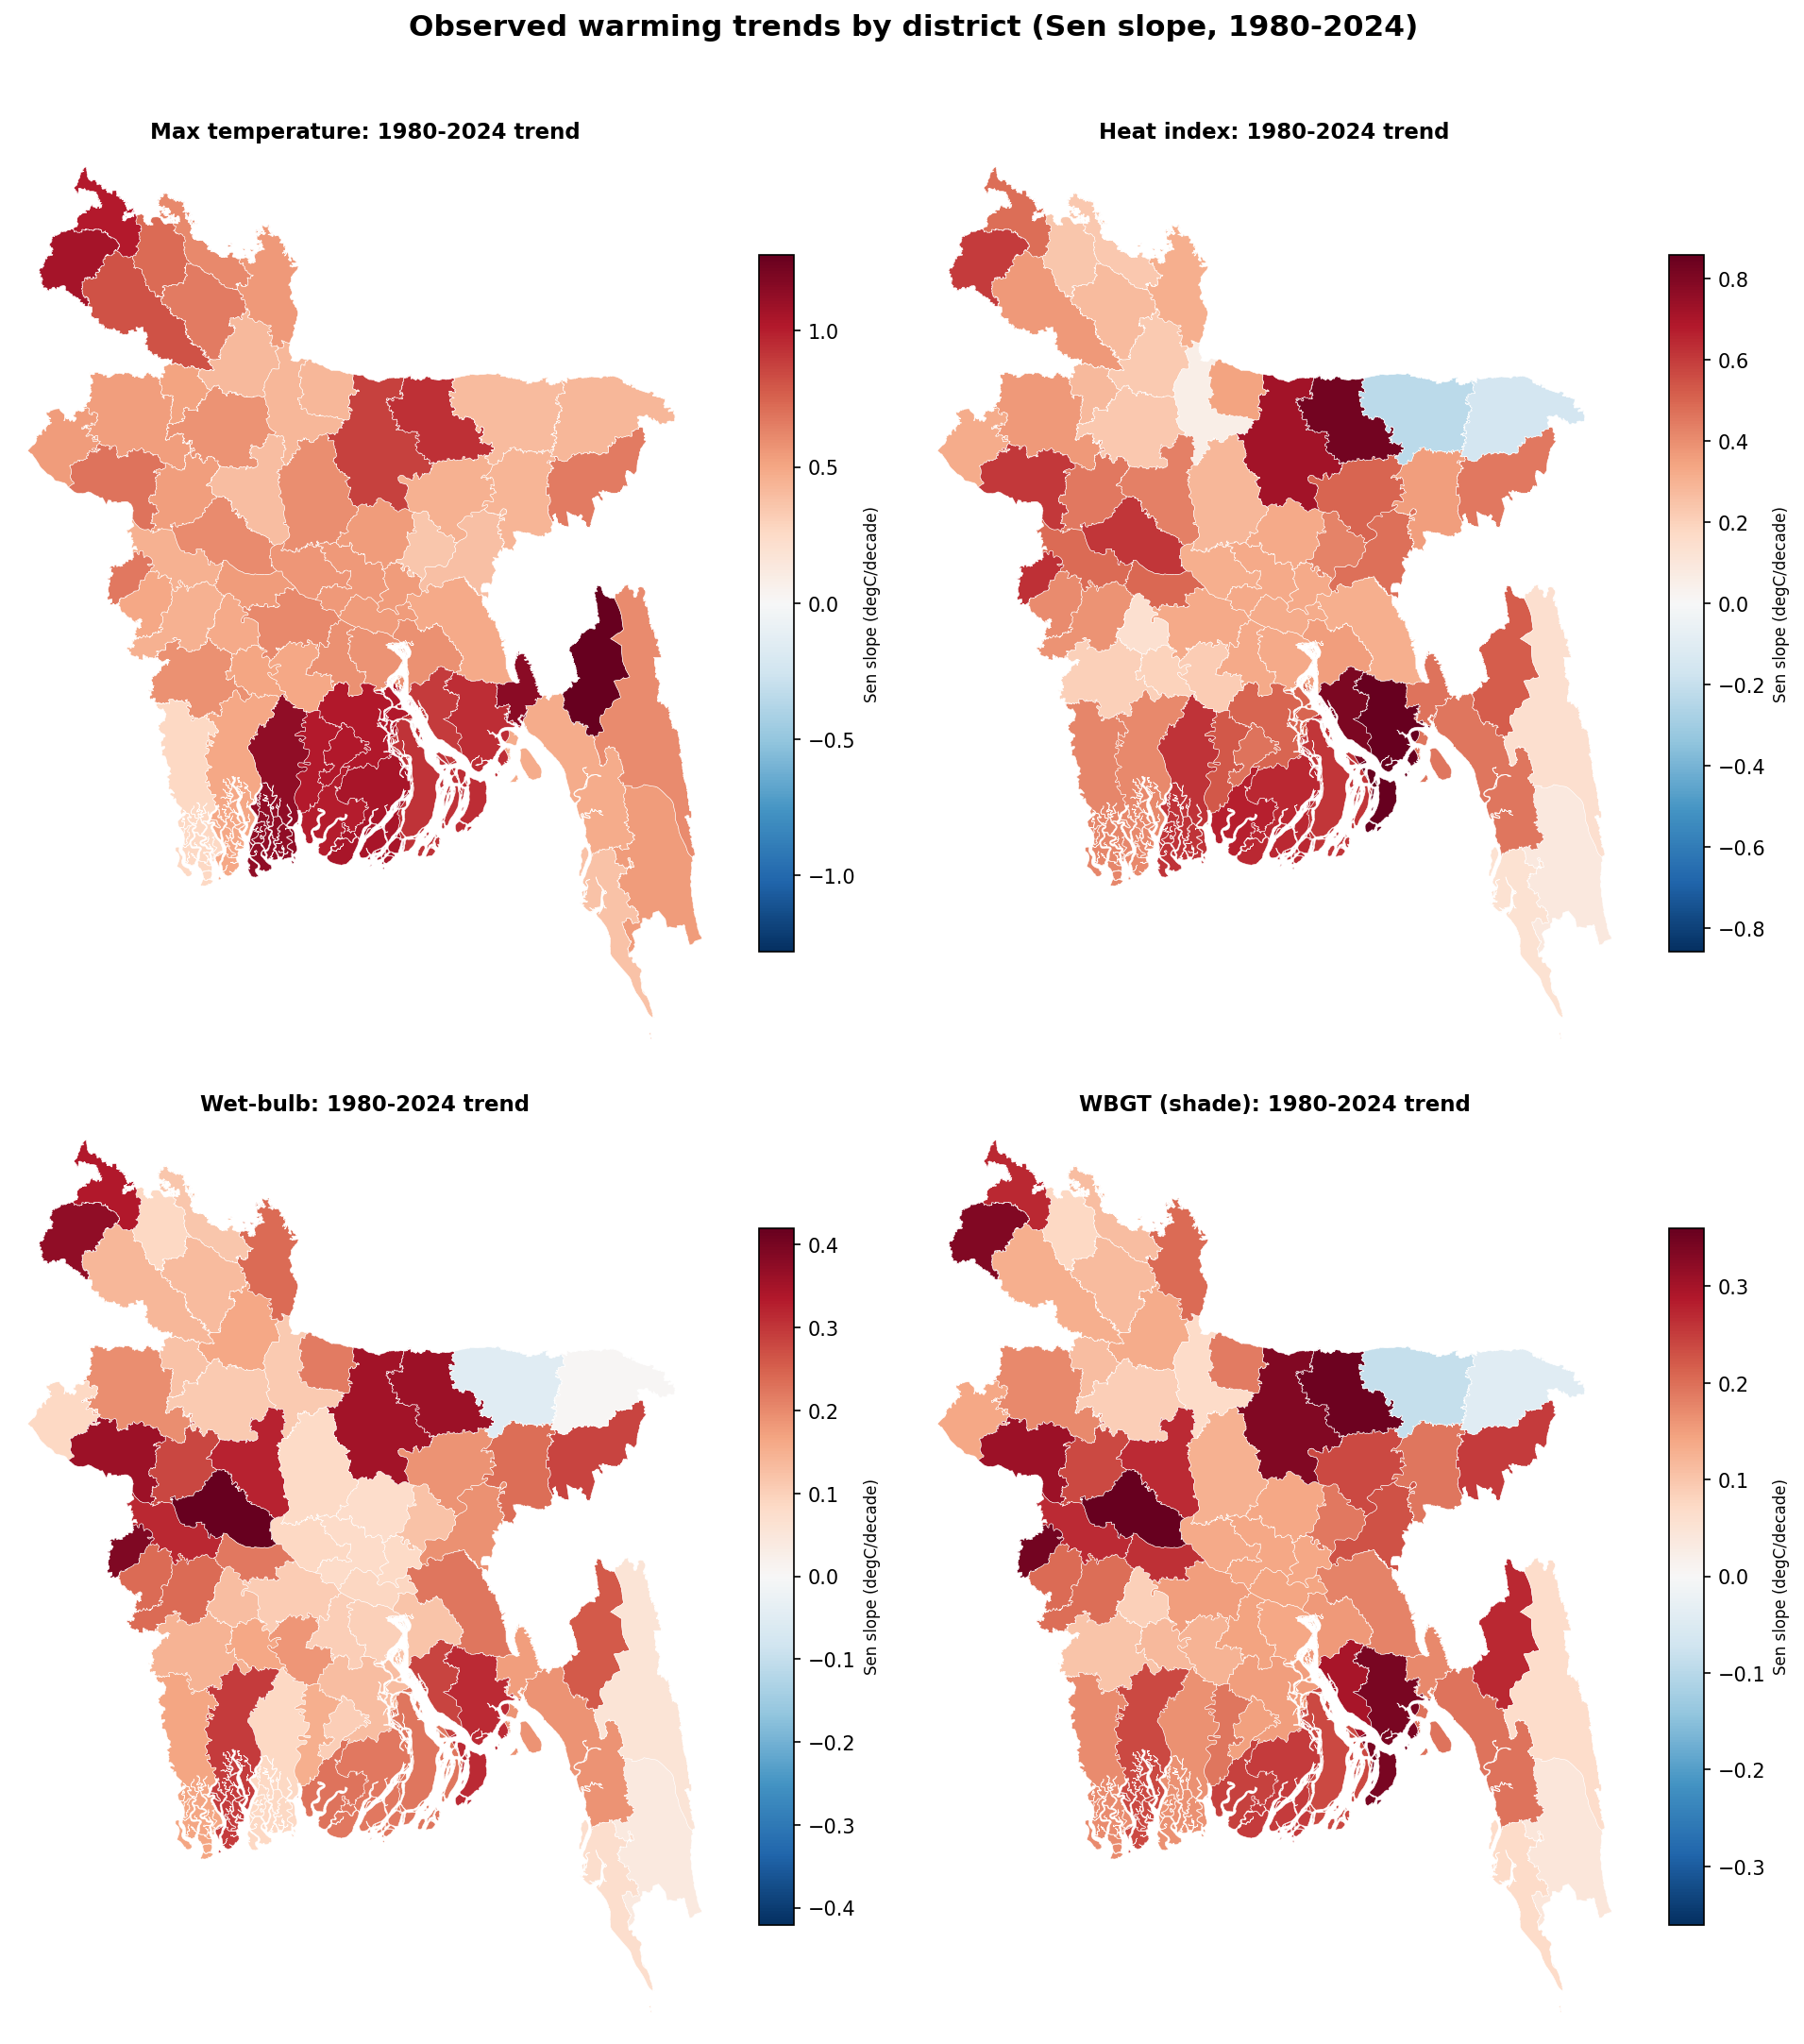
\includegraphics[width=\linewidth]{map_warming_trends.png}
\caption{Observed 1980--2024 warming by district (Theil--Sen slope, $\degC$ per
decade) for maximum temperature, heat index, wet-bulb temperature, and shade
WBGT. Red indicates warming, blue cooling. Values are computed after masking
missing-as-zero early-record days (Section~\ref{sec:trend}).}
\label{fig:maptrend}
\end{figure}

\subsection{Projected 2025--2026 outlook and zonal synthesis}\label{sec:res-proj}
Consistent with the modest observed slopes, the projected year-over-year change
was small: the heat index rose by a median of $+0.038\,\degC$ per year across the
64 districts (range $-0.034$ to $+0.096\,\degC$ per year), the negative values
corresponding to the districts whose 1980--2024 mean-temperature trend is itself
slightly negative. The zonal synthesis (Table~\ref{tab:zonal}) places the highest
projected annual-mean heat index in the Southwest Hot--Dry Zone
($31.0\,\degC$) and the Coastal Humid Heat Zone ($30.6\,\degC$), and the lowest
in the Haor/Wetland Zone ($28.0\,\degC$); sun WBGT peaked in the coastal belt
($25.5\,\degC$). The two continuous-burden conditions reinforce this ordering:
projected cooling degree-days---a proxy for building cooling-energy demand---were
highest in the Southwest Hot--Dry and Coastal Humid Heat zones
($9.1$ and $9.0\,\degC\,\mathrm{d\,d^{-1}}$) and lowest in the Haor/Wetland Zone
($7.0$), while projected wet-bulb temperature, the thermodynamic ceiling on
evaporative cooling, followed the same spatial pattern, peaking in the Coastal
($23.7\,\degC$) and Southwest ($23.6\,\degC$) zones and again reaching its
minimum in the Haor basin ($22.6\,\degC$). The coastal belt therefore emerges as
the zone of greatest combined perceived-heat, humid-heat, and cooling-energy
burden. Figure~\ref{fig:mapmeans} maps all six continuous conditions at district
resolution, confirming the coastal-south concentration of heat, humidity, and
cooling demand. Figure~\ref{fig:threepanel} illustrates the full
record--validation--projection narrative for the Dhaka exemplar, and
Figure~\ref{fig:heatmap} summarises the projected monthly climatology of all six
key conditions across the six zones, exposing their distinct seasonal
signatures. Figure~\ref{fig:envelope} shows the district spread within the hottest
(Southwest) zone.

\begin{table}[htbp]
\centering
\caption{Projected annual-mean thermal indices by climatic zone (zone mean, with
the across-district minimum and maximum in parentheses). Values in $\degC$ except
CDD ($\degC$\,d\,d$^{-1}$).}
\label{tab:zonal}
\begin{tabular}{lcccc}
\toprule
Zone & Heat index & WBGT (sun) & Wet-bulb & CDD \\
\midrule
1. Northwest Extreme Heat & 29.6 (28.4--30.7) & 24.7 & 22.9 & 8.3 \\
2. Central Urban Heat     & 29.6 (29.3--30.9) & 24.8 & 22.8 & 8.8 \\
3. Southwest Hot--Dry     & 31.0 (30.6--31.9) & 25.5 & 23.6 & 9.1 \\
4. Coastal Humid Heat     & 30.6 (29.5--31.5) & 25.5 & 23.7 & 9.0 \\
5. Haor/Wetland Humid     & 28.0 (26.0--29.5) & 24.3 & 22.6 & 7.0 \\
6. Hill Tract             & 29.9 (29.3--30.3) & 25.4 & 23.5 & 8.6 \\
\bottomrule
\end{tabular}

\end{table}

\begin{figure}[htbp]
\centering
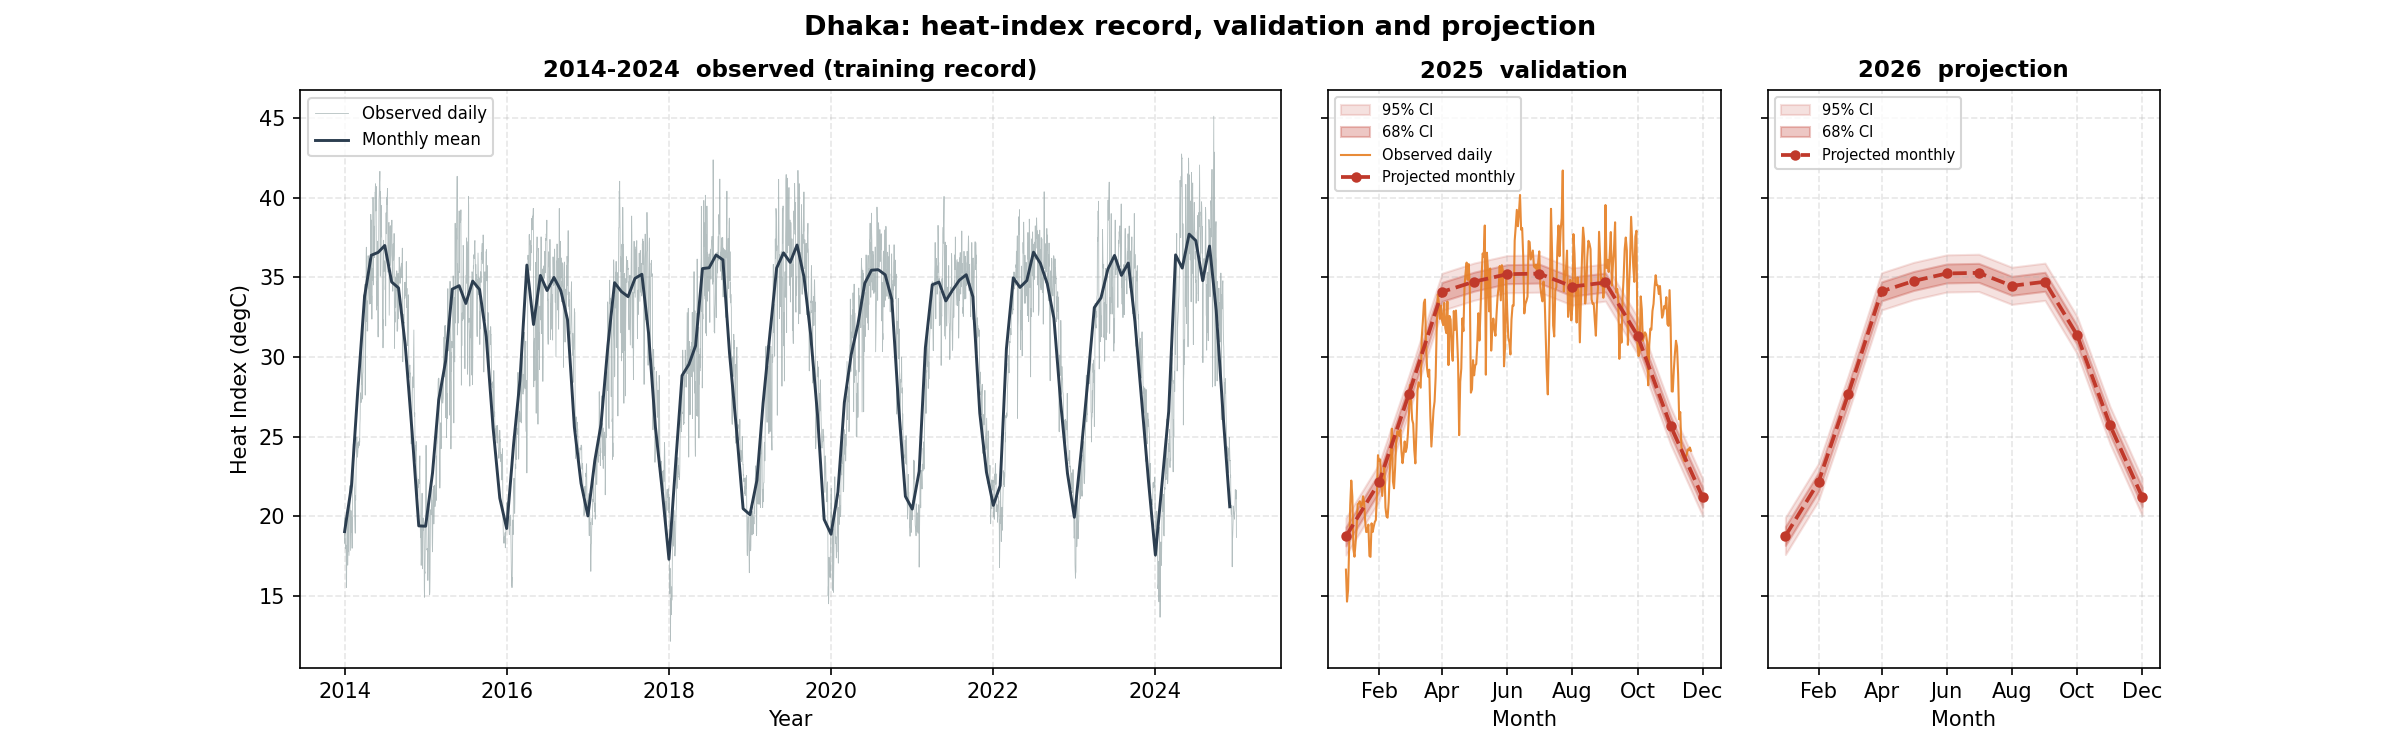
\includegraphics[width=\linewidth]{threepanel_Dhaka_heat_index.png}
\caption{Heat-index record, validation, and projection for the Dhaka exemplar:
(left) observed daily heat index 2014--2024 with the monthly mean; (centre) the
2025 validation year, observed daily versus the monthly projection with 68\% and
95\% confidence bands; (right) the 2026 monthly projection with confidence cloud.}
\label{fig:threepanel}
\end{figure}

\begin{figure}[htbp]
\centering
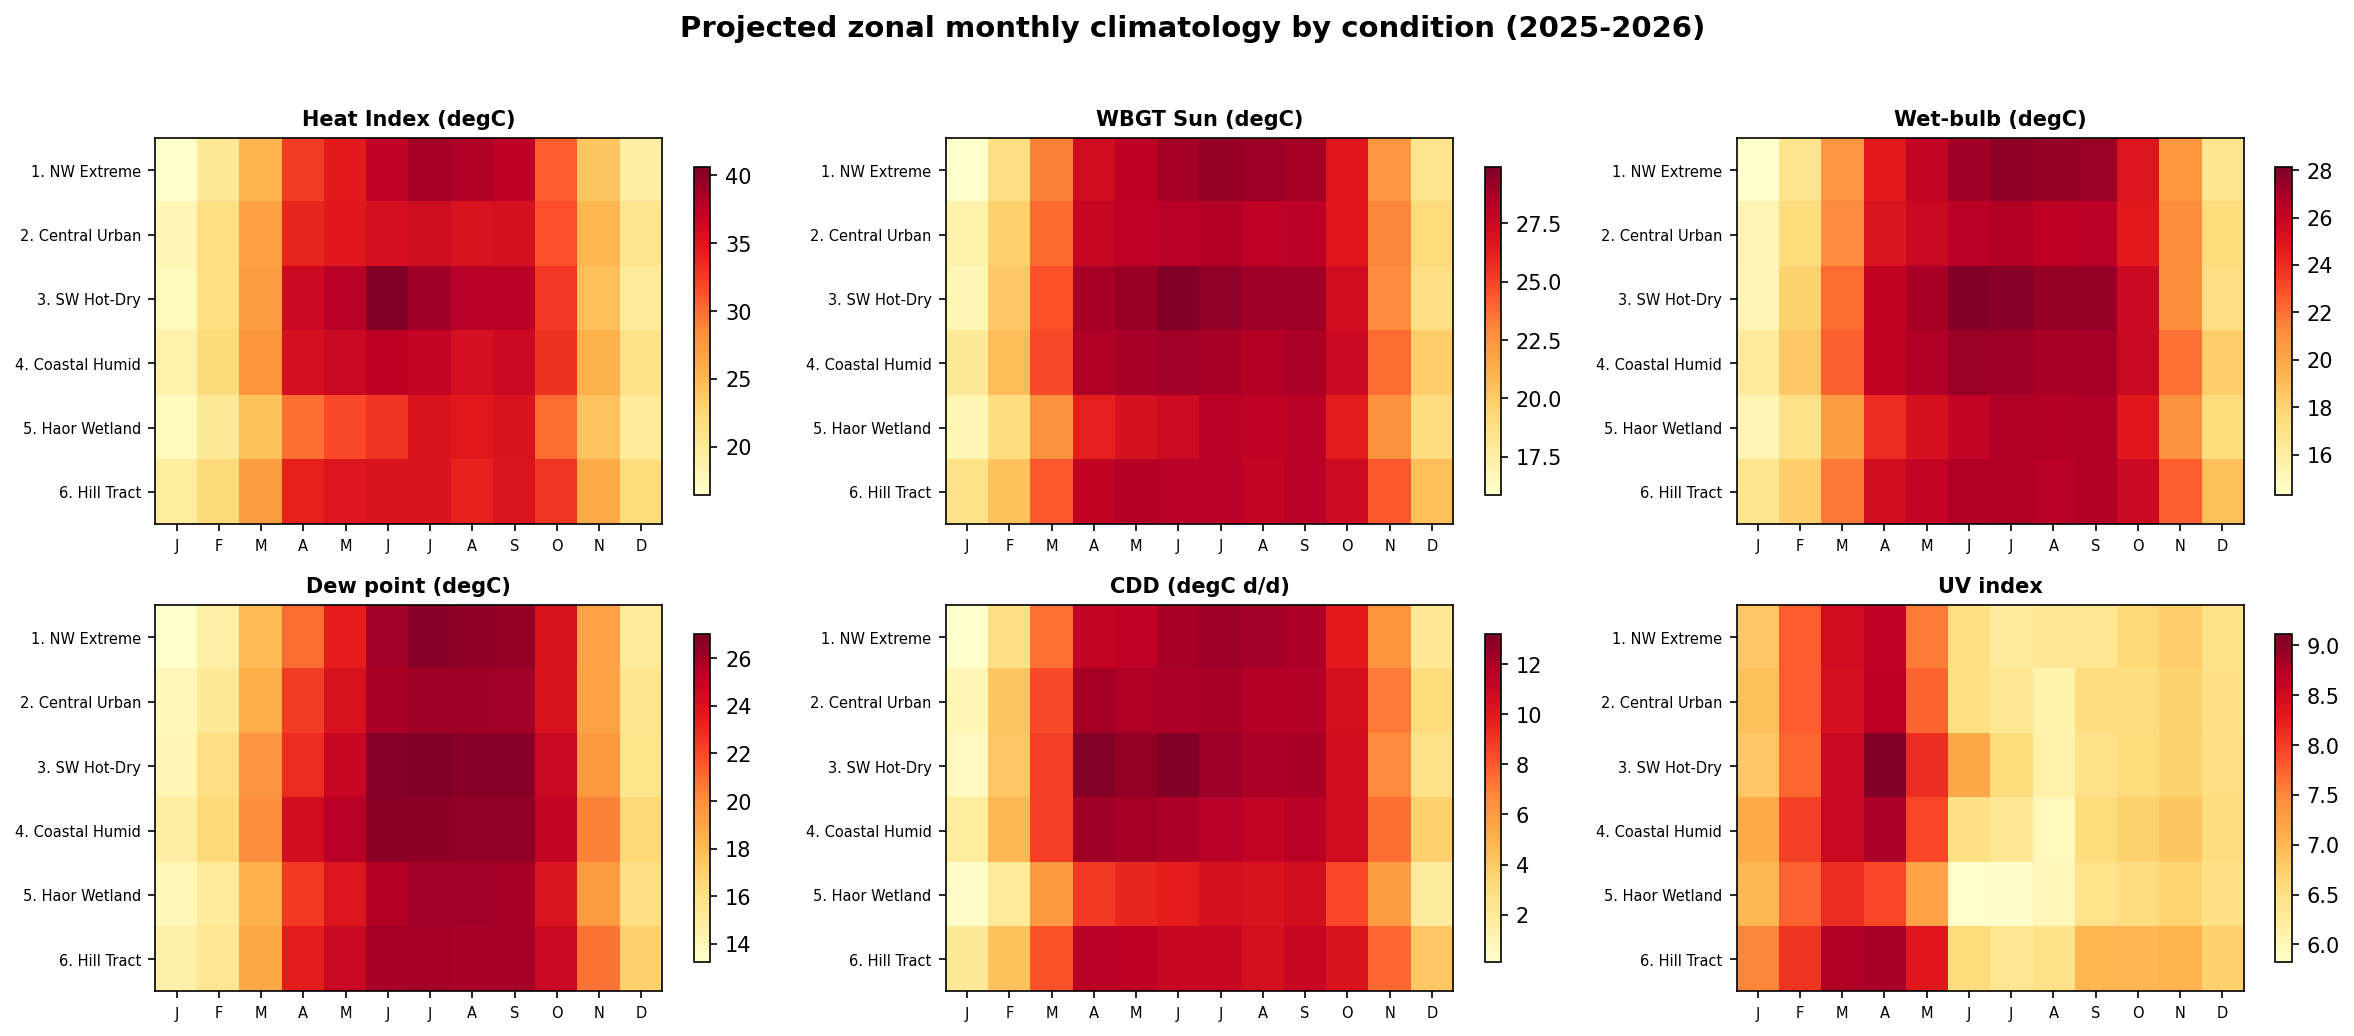
\includegraphics[width=\linewidth]{heatmap_multi.png}
\caption{Projected zonal monthly climatology for six heat-stress conditions
(heat index, sun WBGT, wet-bulb temperature, dew point, cooling degree-days, and
UV index). The temperature-driven conditions peak in the pre-monsoon to monsoon
window, whereas the UV index peaks in the dry pre-monsoon (March--April) and
falls during the cloudy monsoon --- a distinct, radiation-driven seasonality.}
\label{fig:heatmap}
\end{figure}

\begin{figure}[htbp]
\centering
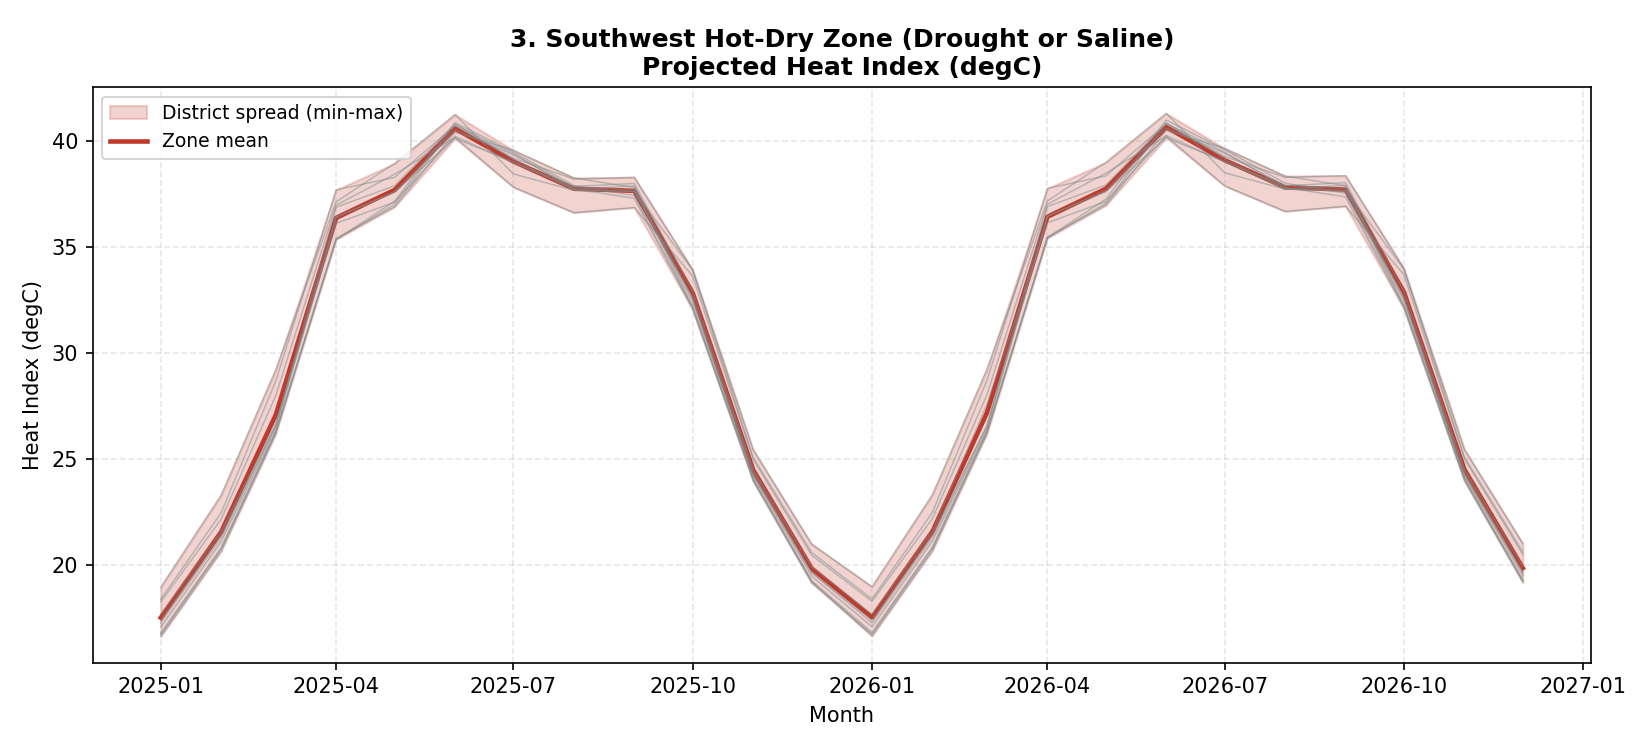
\includegraphics[width=0.85\linewidth]{zone3_heat_index.png}
\caption{Projected heat index for the Southwest Hot--Dry Zone: the zone mean and
the min--max envelope across member districts, illustrating within-zone spread.}
\label{fig:envelope}
\end{figure}

\begin{figure}[htbp]
\centering
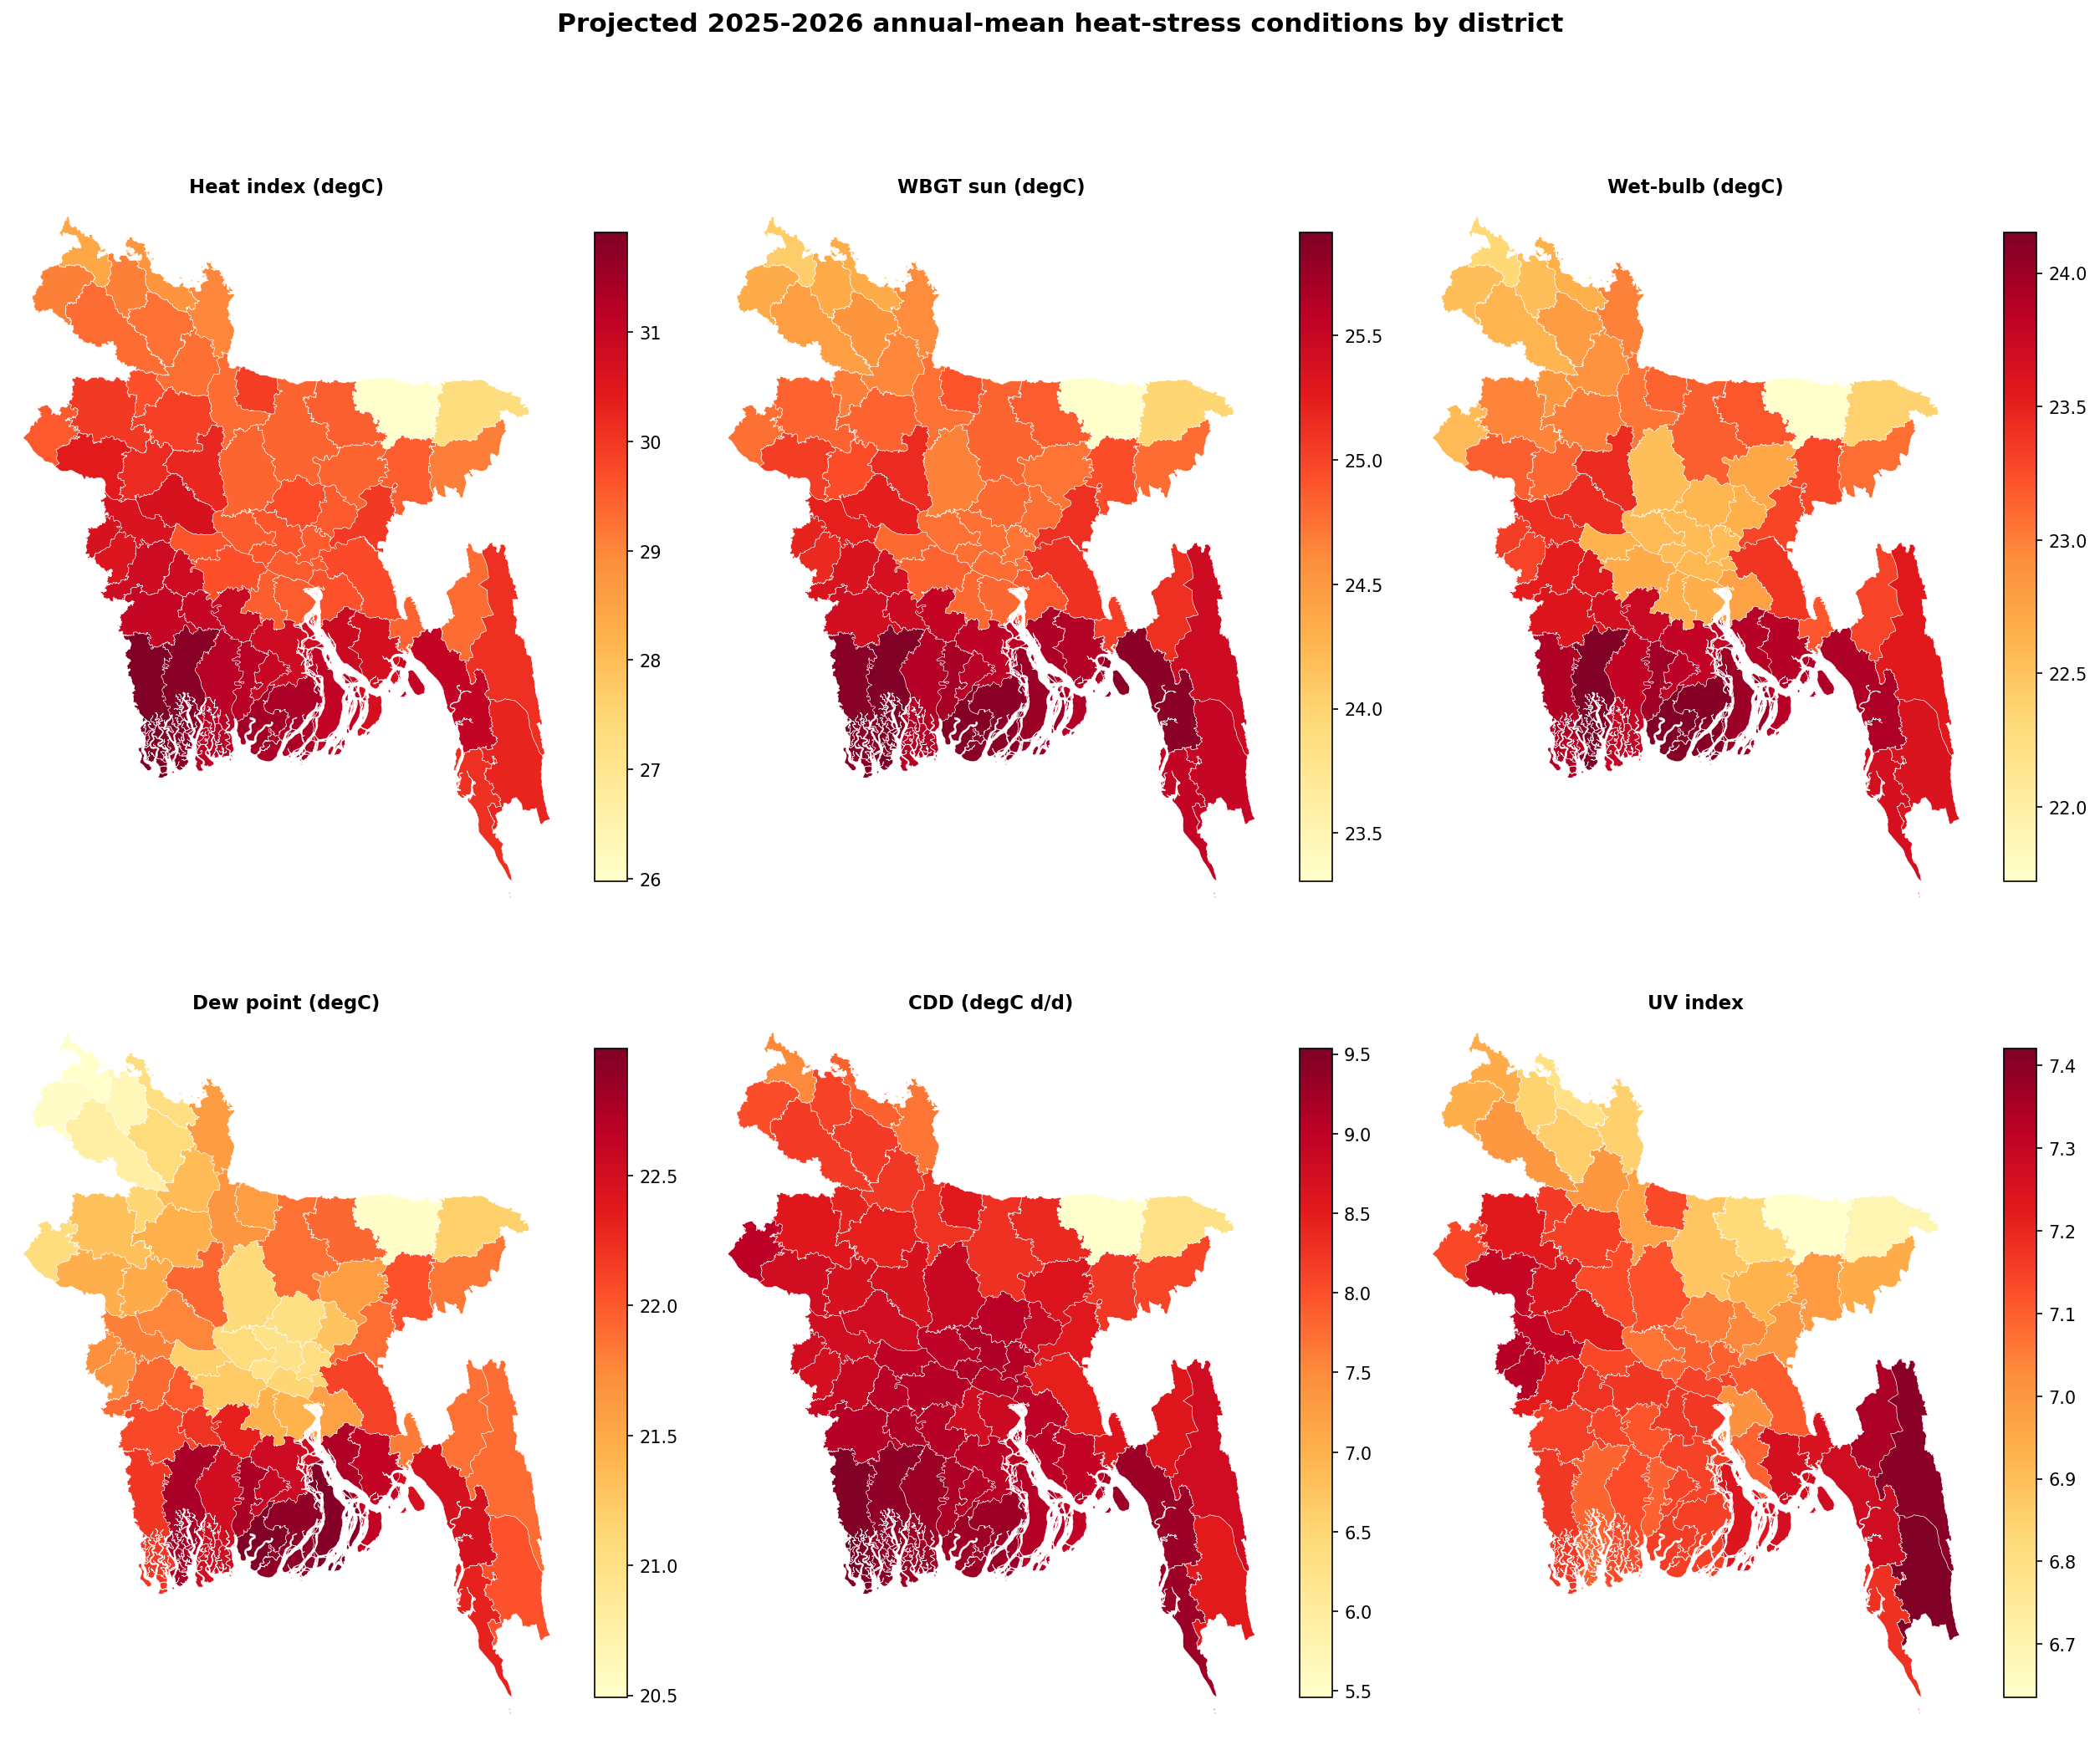
\includegraphics[width=\linewidth]{map_projected_means.png}
\caption{Projected 2025--2026 annual-mean heat-stress conditions by district:
heat index, sun WBGT, wet-bulb temperature, dew point, cooling degree-days, and
UV index. Every condition is shown at full district resolution rather than
aggregated to zones.}
\label{fig:mapmeans}
\end{figure}

\subsection{Operational risk categories}\label{sec:res-categories}
Mapping the projected fields onto their risk-category systems yields a
policy-facing summary of the seven conditions (Table~\ref{tab:catdist}). Under
monthly-mean heat index, projected months split between Comfortable (37.8\%) and
Extreme Caution (51.8\%), with the intermediate Caution class at 10.2\% and the
Danger class essentially absent (0.1\%)---the latter a direct consequence of
categorising monthly means rather than daily peaks. Outdoor WBGT was
predominantly Low (59.0\%) to Moderate (37.0\%), reaching the High class in
3.9\% of months, while indoor (shade) WBGT rarely left the Low class (79.8\%).
The UV signal was the most consistently hazardous condition: 75.5\% of projected
months fall in the WHO High class and a further 20.4\% in Very High. Dew-point
moisture stress was also severe, with 45.5\% of months in the Extremely
Oppressive class. Across zones, the Southwest Hot--Dry Zone carried the largest
Extreme-Caution share for heat index (57.5\%) and the only appearance of the
Danger class (0.8\%), whereas the Haor/Wetland Zone was the mildest (35.4\%
Extreme Caution); Figure~\ref{fig:catzone} shows the full zonal composition and
Figure~\ref{fig:maphazard} maps, for each district, the number of months per year
spent at or above each condition's hazard threshold. The months-per-year view
resolves the strong spatial and seasonal gradients that a dominant-class map
obscures: the coastal south endures dew-point levels in the Extremely Oppressive
class for roughly seven to eight months per year against three to four in the
northwest, and very-high UV persists longest in the south.

Critically, the categorical layer validated well against observed 2025
(Table~\ref{tab:catval}): exact-class agreement ranged from 81.5\% (UV) to
89.8\% (heat-index comfort), and agreement to within one adjacent class reached
100\% for all five categorised conditions. The projection therefore reproduces
not only the continuous fields but also their operational risk classification.

\begin{table}[htbp]
\centering
\caption{Projected risk-category distribution (share of projected
district-months, 2025--2026, 64 districts). Only populated categories are shown.}
\label{tab:catdist}
\begin{tabular}{llr}
\toprule
Condition & Category & Share (\%) \\
\midrule
Heat-index comfort        & Comfortable             & 37.8 \\
                          & Caution                 & 10.2 \\
                          & Extreme Caution         & 51.8 \\
                          & Danger                  & 0.1 \\
\midrule
WBGT (sun, outdoor)       & Low                     & 59.0 \\
                          & Moderate                & 37.0 \\
                          & High                    & 3.9 \\
\midrule
WBGT (shade, indoor)      & Low                     & 79.8 \\
                          & Moderate                & 20.2 \\
\midrule
UV (WHO)                  & Moderate                & 4.2 \\
                          & High                    & 75.5 \\
                          & Very High               & 20.4 \\
\midrule
Dew-point moisture stress & Comfortable             & 19.7 \\
                          & Slightly Humid          & 6.6 \\
                          & Humid                   & 16.3 \\
                          & Very Humid / Oppressive & 11.9 \\
                          & Extremely Oppressive    & 45.5 \\
\bottomrule
\end{tabular}

\end{table}

\begin{table}[htbp]
\centering
\caption{Categorical validation against observed 2025: exact-class agreement and
agreement to within one adjacent class, pooled over district-months.}
\label{tab:catval}
\begin{tabular}{lccc}
\toprule
Condition & $n$ & Exact-class (\%) & Within one class (\%) \\
\midrule
Heat-index comfort         & 704 & 89.8 & 100.0 \\
WBGT (sun, outdoor)        & 704 & 84.1 & 100.0 \\
WBGT (shade, indoor)       & 704 & 88.8 & 100.0 \\
UV (WHO)                   & 704 & 81.5 & 100.0 \\
Dew-point moisture stress  & 704 & 87.1 & 100.0 \\
\bottomrule
\end{tabular}

\end{table}

\begin{figure}[htbp]
\centering
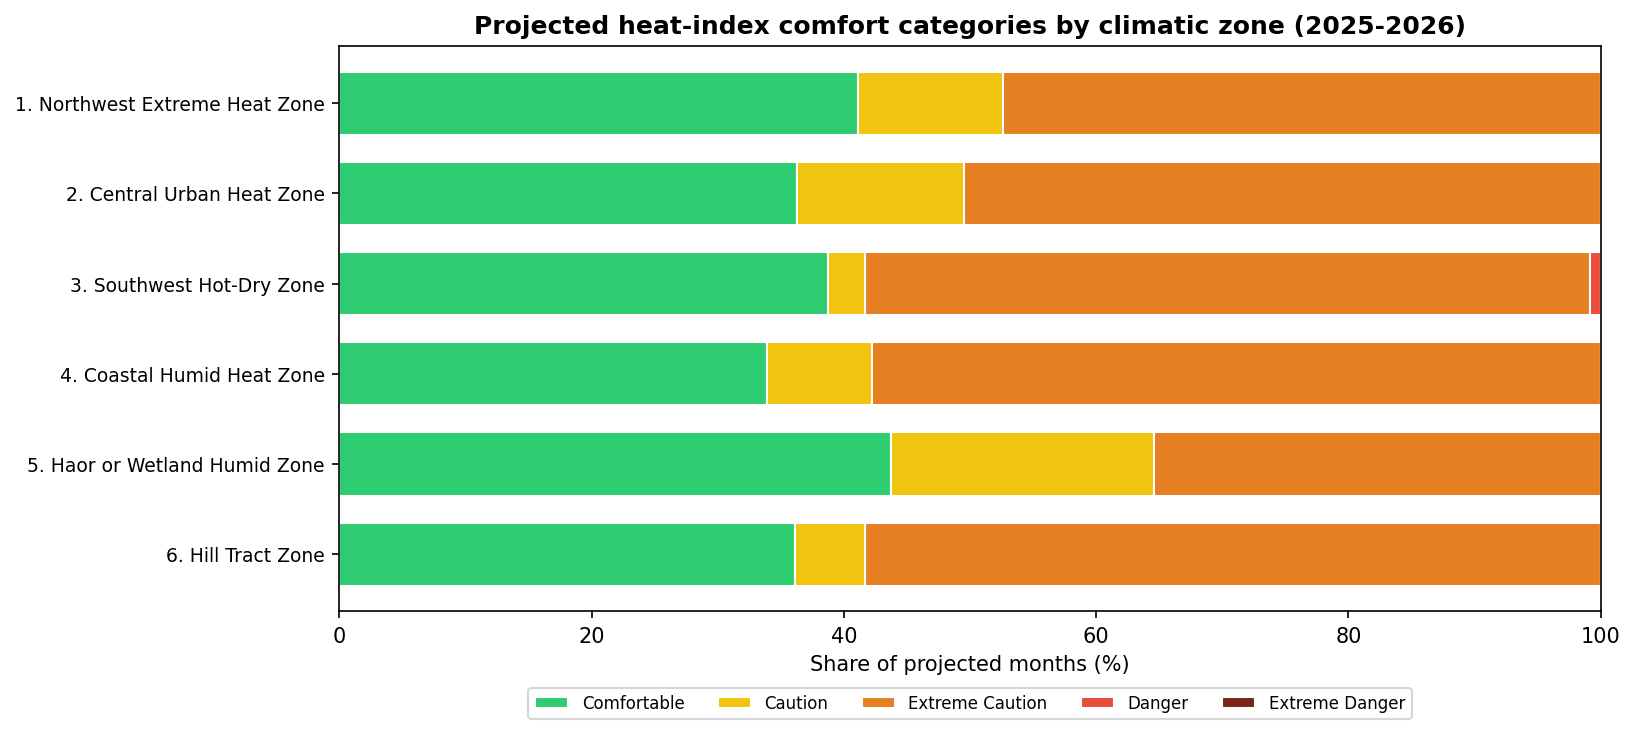
\includegraphics[width=\linewidth]{category_heatindex_by_zone.png}
\caption{Projected heat-index comfort categories by climatic zone (share of
projected months, 2025--2026). The Southwest Hot--Dry Zone carries the largest
Extreme-Caution share and the only Danger occurrences; the Haor/Wetland Zone is
mildest.}
\label{fig:catzone}
\end{figure}

\begin{figure}[htbp]
\centering
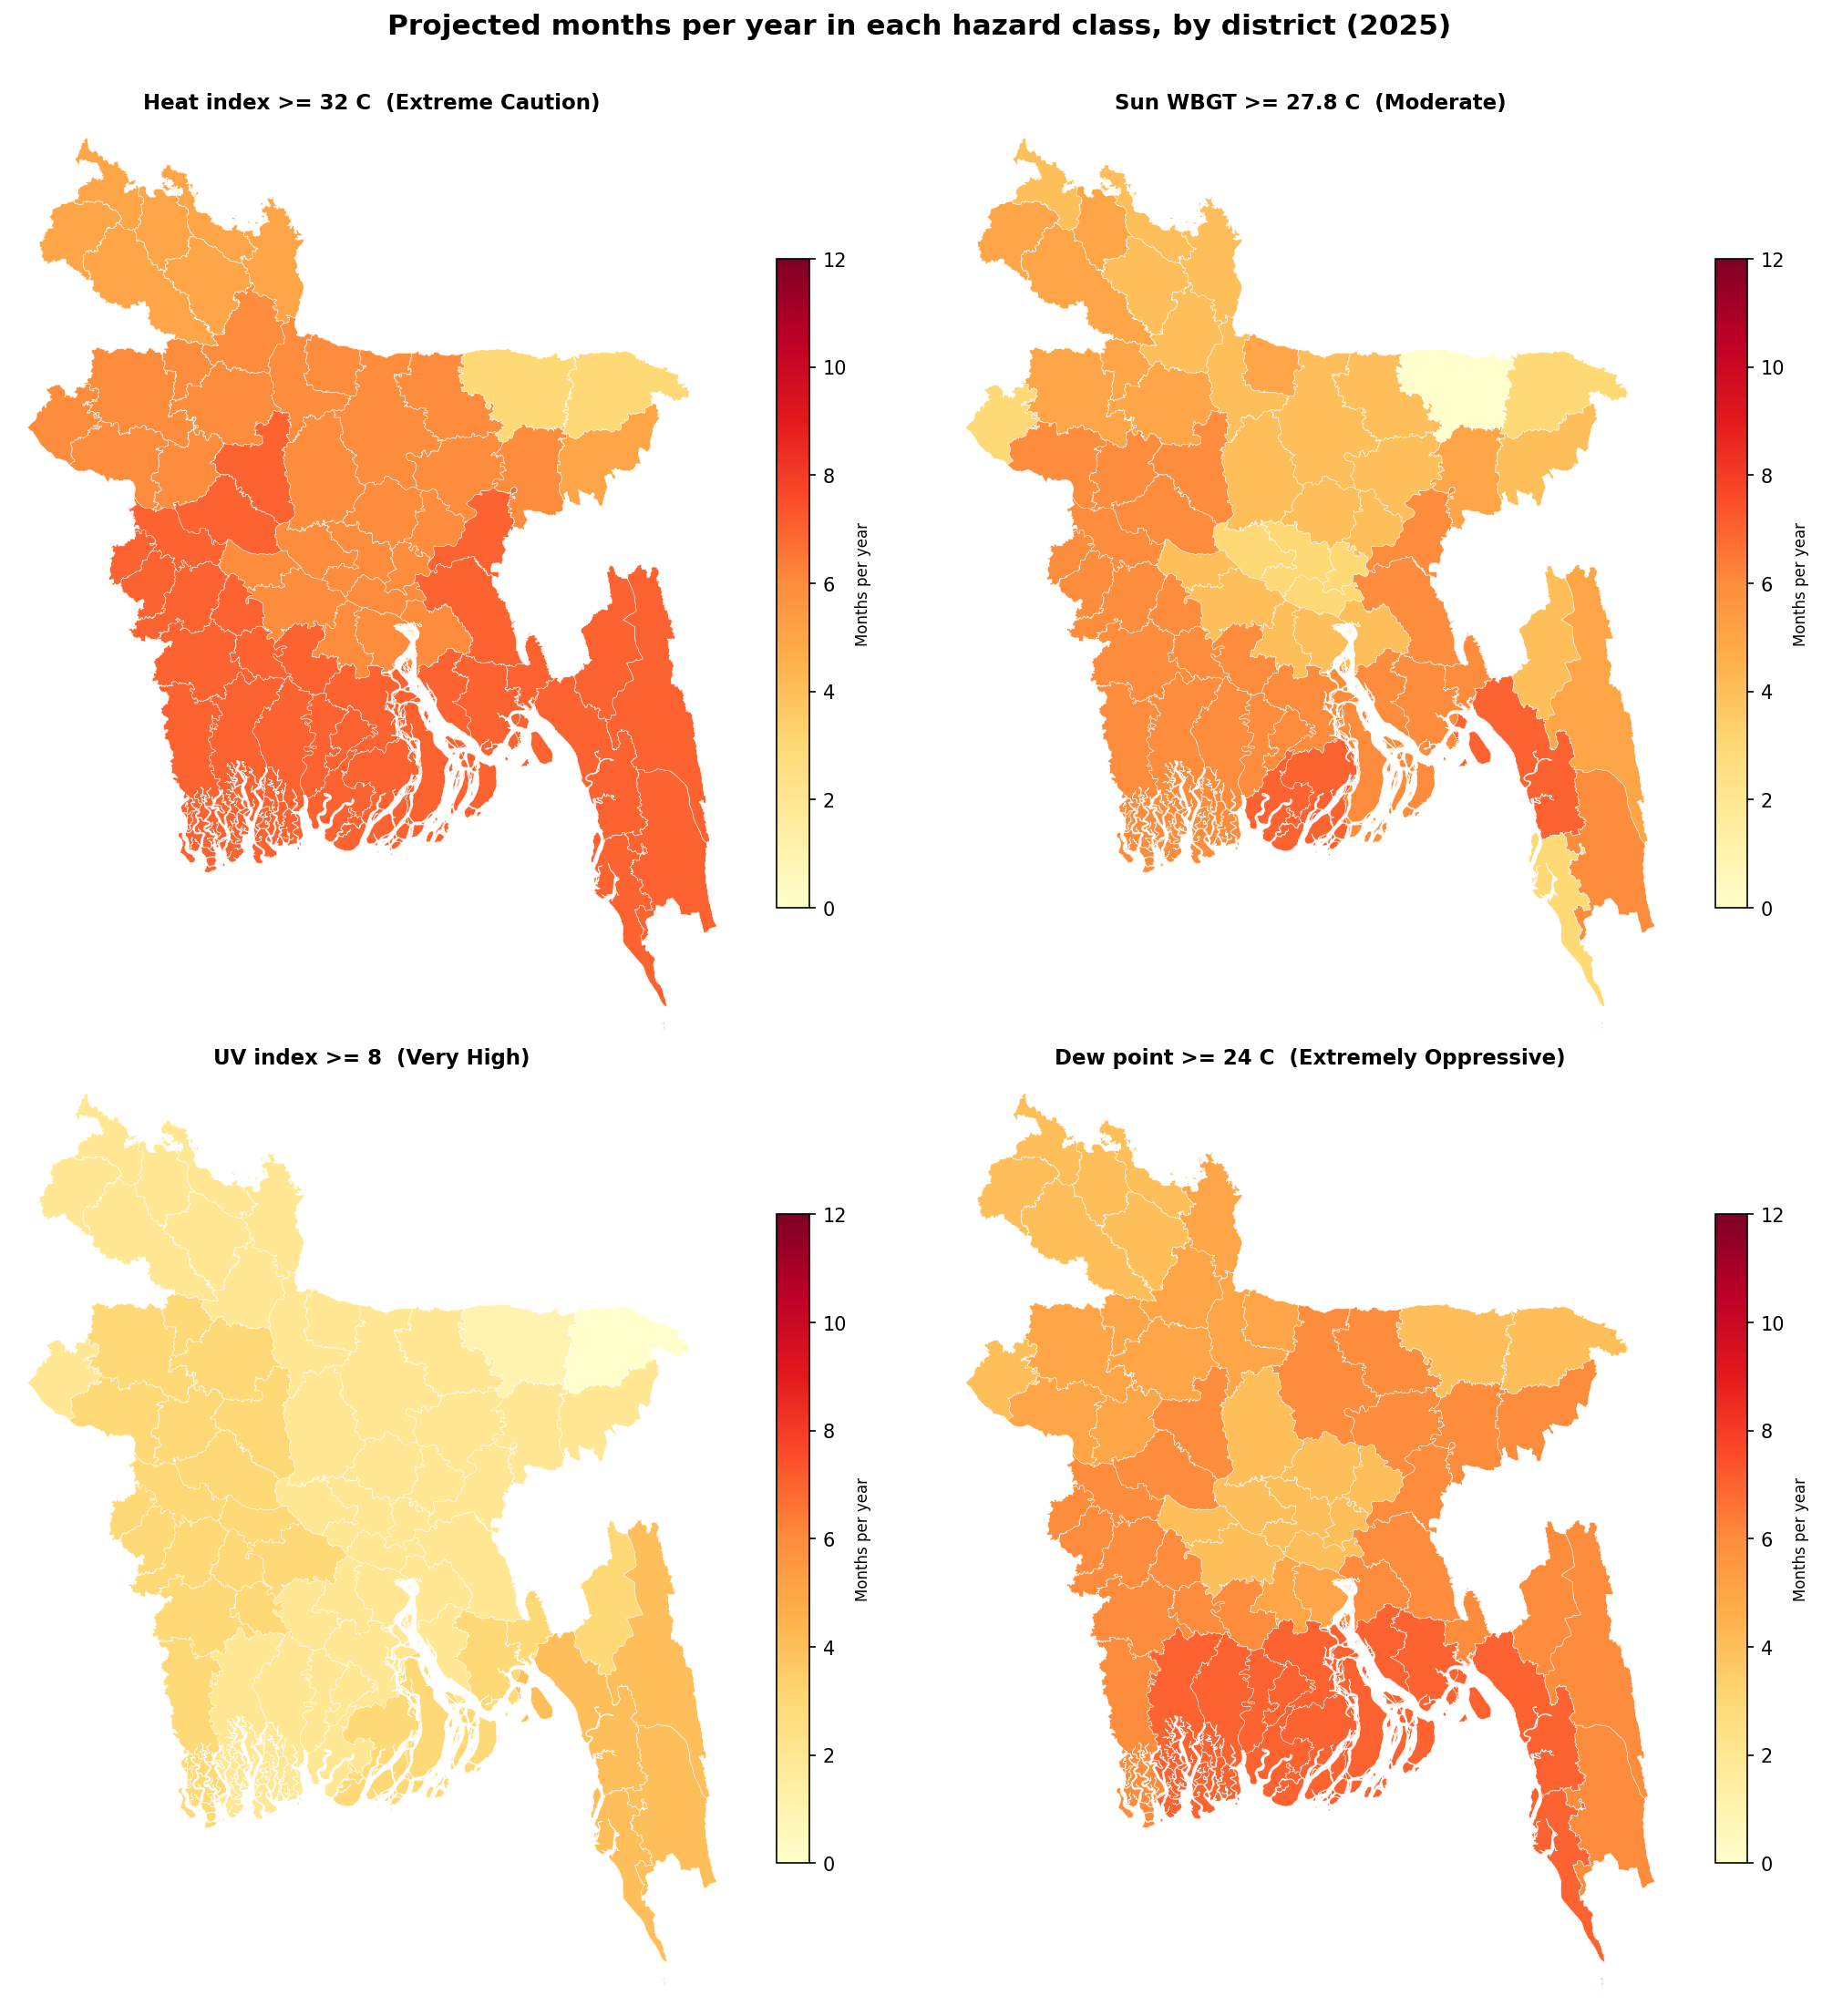
\includegraphics[width=\linewidth]{map_hazard_months.png}
\caption{Projected number of months per year (of 12) that each district spends at
or above a hazard threshold, for heat index ($\ge32\,\degC$, Extreme Caution),
sun WBGT ($\ge27.8\,\degC$, Moderate), UV ($\ge8$, Very High), and dew point
($\ge24\,\degC$, Extremely Oppressive). This months-per-year measure preserves the
seasonal and spatial structure that a single dominant-class map collapses.}
\label{fig:maphazard}
\end{figure}

\subsection{Projection uncertainty}\label{sec:res-uncert}
The first-order error propagation yielded confidence bands that are approximately
constant across the 24-month horizon, reflecting the dominance of the seasonal
model's error over the small trend extrapolation. For the Dhaka exemplar, the
95\% heat-index band was $\pm1.17\,\degC$, the wet-bulb band $\pm0.99\,\degC$, and
the sun-WBGT band $\pm0.76\,\degC$. These bands exceed the projected
inter-annual trend signal by more than an order of magnitude, and this
relationship is stated explicitly to caution against over-interpreting small
year-to-year differences in the projection.

%% ===========================================================================
\section{Discussion}\label{sec:discussion}

\subsection{Principal findings}
This study delivers district-resolved, uncertainty-aware near-term projections of
seven temperature-correlated heat-stress conditions for all 64 districts of
Bangladesh, together with a leakage-free external validation against independent
2025 observations. The recomputed thermal indices validated strongly---heat
index, wet-bulb temperature, and WBGT all at median $R^{2}\ge0.95$---and, when
mapped onto their operational risk classes, reproduced the observed 2025 class in
$81$--$90\%$ of district-months exactly and in $100\%$ to within one adjacent
class. Because the indices are computed from the projected primary variables
rather than predicted directly, this accuracy is achieved without target leakage
and while preserving the physical coupling among temperature, humidity, and
radiation. This validated, multi-index projection extends prior Bangladeshi
heat-projection work that has largely treated single indices in isolation---most
notably the heat-index appraisal of \citet{rahman2021} and the WBGT trend analysis
of \citet{kamal2024scientific}---and complements single-algorithm forecasting
precedents such as \citet{mollah2026mlheatindex} and \citet{islam2026enso} by
covering all seven conditions jointly and validating them out-of-sample.

\subsection{Skill must be interpreted correctly}
A central and deliberately transparent result is that, although the ensembles
comfortably outperform a seasonal-naive baseline, they are essentially at parity
with monthly climatology (positive skill in only $\sim\!32\%$ of
district--variable cases). This is expected rather than disappointing: at monthly
resolution the tropical seasonal cycle dominates the variance, and any competent
learner reconstructs the climatological annual march that climatology also
encodes. The contribution of the framework is therefore not a reduction in
monthly error but the provision of a spatially complete, uncertainty-quantified,
and trend-consistent projection---including physiologically relevant indices and
their operational risk classes---that a bare climatology cannot supply. We state
this explicitly to discourage over-claiming predictive skill that the data do not
support. This transparency deliberately contrasts with the common practice of
reporting high absolute accuracy---for instance the $R^{2}$ values near $0.99$ and
$0.88$--$0.97$ reported for Bangladeshi heat-index and temperature prediction by
\citet{mollah2026mlheatindex} and \citet{islam2026enso}---without benchmarking
against a climatological reference, which can make routine seasonal reconstruction
appear as genuine forecasting skill.

\subsection{Physical and spatial interpretation}
The observational analysis reveals a coherent but spatially structured warming
signal. Maximum temperature increased in every district (median $+0.56\,\degC$
per decade) while minimum temperature remained essentially flat (median
$+0.02\,\degC$ per decade), implying a widening diurnal temperature range across
much of the country---a pattern with distinct implications for daytime heat
exposure and nighttime physiological recovery. Humid-heat indices (heat index,
wet-bulb, WBGT) rose in $57$--$58$ of 64 districts, confirming that the warming is
not purely a dry-bulb phenomenon. Spatially, the Southwest Hot--Dry and Coastal
Humid Heat zones carry the greatest projected burden across perceived heat,
humid heat, and cooling-energy demand, whereas the elevated Haor/Wetland basin is
consistently mildest; the coastal belt in particular combines the highest
wet-bulb temperatures and cooling degree-days, marking it as a priority region.
These patterns matter physiologically: the elevated coastal wet-bulb burden erodes
the evaporative margin that \citet{raymond2020} identified as the hard limit of
human heat tolerance, in the same coastal belt where \citet{tanim2024heat} found
the steepest historical rise in heat discomfort. The widening diurnal range is also
epidemiologically salient, since reduced nighttime cooling impairs physiological
recovery and compounds the heatstroke-mortality and labour-capacity risks
documented for Bangladesh and for outdoor workers more broadly
\citep{miah2026,flouris2022}.

\subsection{Operational risk categories and their message}
Translating the projections into established risk classes sharpens the
public-health narrative. The UV signal is the most uniformly hazardous condition:
essentially the entire country falls in the WHO High class or above throughout the
projection, and dew-point moisture stress reaches the Extremely Oppressive class
in almost half of all projected months. Heat-index comfort is dominated by the
Extreme Caution class in the warm season, while the Danger class is essentially
absent---a direct and important consequence of categorising monthly means rather
than daily maxima (Section~\ref{sec:conditions}), which the categories must be
read against. The nationwide reach of the UV and humidity hazards, contrasted with
the more spatially variable heat-index and WBGT burden, argues for differentiated
adaptation responses: the near-universal High-to-Very-High UV exposure calls for
the sun-protection measures codified in the WHO UV-index guidance \citep{who2002},
whereas the humid-heat burden is better addressed through the WBGT-based
occupational-safety framework of ISO~7243 \citep{iso7243_2017,parsons2006}, whose
relevance is amplified by the large humid-heat labour losses estimated for South
Asian outdoor workers \citep{parsons2021labor}.

\subsection{Methodological reflections}
Three design choices proved consequential. First, recomputing indices from
projected primary variables (rather than modelling them directly) both prevents
target leakage and guarantees internal physical consistency of the projected
fields. Second, the detrend--residual--retrend construction resolves a failure
mode of tree ensembles---their inability to extrapolate a calendar-year
feature---so that projected years evolve with the observed climate trend instead
of collapsing onto the last training year; imposing the robust 1980--2024 Sen
slope additionally keeps the projection consistent with the manuscript's own
trend analysis by construction. Third, the district choropleths exposed a
data-quality problem (early-record missing values encoded as zero) that
zonal-median summaries had masked, underscoring the value of full-resolution
spatial diagnostics and prompting the physical-floor correction described in
Section~\ref{sec:trend}.

\subsection{Limitations}
Several limitations bound the interpretation. (i)~The projection horizon is
deliberately restricted to 24 months; because the re-added trend is small relative
to the projection uncertainty (the $95\%$ heat-index band exceeds the annual
trend signal by more than an order of magnitude), longer horizons would add
deterministic drift without validatable information. (ii)~Working at monthly-mean
resolution necessarily compresses daily extremes, so the risk categories describe
typical monthly conditions and systematically under-represent short-duration
dangerous events; a daily-resolution extension is the natural next step.
(iii)~A composite heatstroke-hazard index was implemented but excluded from
predictive results for negative out-of-sample skill, and is reported only
descriptively. (iv)~All meteorological inputs derive from a single commercial
reanalysis-blended source; despite strong 2025 validation, independent
station-based corroboration would strengthen confidence, and the early-record
inhomogeneity in a subset of districts (mitigated here by masking) illustrates the
sensitivity of long-run trends to input quality. (v)~The models add little skill
over climatology at monthly scale, as discussed above. The 24-month horizon is
complementary to, rather than competitive with, the multi-decadal CMIP6 projections
available for Bangladesh and the wider region \citep{khatun2024,kushwaha2026humidex}:
those studies bound the long-term trajectory under emission scenarios, whereas the
present framework supplies the near-term, district-resolved, externally validated
detail that dynamical downscaling cannot yet deliver at this resolution.

\subsection{Outlook}
Several extensions follow naturally. A daily-resolution implementation would
recover the short-duration extremes that monthly means smooth away and let the risk
categories reflect daily peaks---the regime in which the heatstroke indicator
excluded here may regain skill \citep{ehsan2026extremeheat}. Coupling the projected
fields with health-surveillance and cooling-energy records would convert the
physical outlook into quantified public-health and infrastructure burdens
\citep{miah2026}. Methodologically, the framework can absorb recent advances in the
individual conditions---reanalysis-based UV retrieval \citep{teggi2026uvindex} and
attention-based dew-point models with explainability \citep{abdullah2025xai}---and
its near-term projections can be systematically benchmarked against CMIP6 dynamical
downscaling \citep{khatun2024} to bridge near-term operational forecasting and
long-term climate projection.

%% ===========================================================================
\section{Conclusion}\label{sec:conclusion}
This study introduced the Temperature-Correlated Conditions (TCC) framework and
applied it to project seven physiologically and operationally relevant heat-stress
conditions across all 64 districts of Bangladesh. By training gradient-boosting
ensembles on the 2014--2024 record with future-known seasonal features,
re-imposing the observed 1980--2024 trend, and recomputing every thermal index
from the projected primary variables, the framework produced district-level
24-month projections that validated strongly against independent 2025
observations---median $R^{2}$ of $0.95$--$0.98$ for the key indices, with
operational risk classes reproduced to within one category in $100\%$ of
district-months.

The observational analysis revealed a coherent but spatially structured warming
signal: maximum temperature rose in every district (median $+0.56\,\degC$ per
decade) while minimum temperature remained essentially flat, implying a widening
diurnal temperature range, and the humid-heat indices increased across most of the
country. Spatially, the coastal and southwestern zones emerged as the areas of
greatest combined perceived-heat, humid-heat, and cooling-energy burden, whereas
ultraviolet and oppressive-humidity hazards were effectively nationwide. Crucially,
the ensembles were found to be at parity with monthly climatology; the framework's
contribution is therefore not improved monthly accuracy but a spatially complete,
uncertainty-aware, and trend-consistent outlook---delivered at full district
resolution---that supports targeted heat-adaptation planning. One indicator,
heatstroke risk, was excluded from the predictive results for a lack of
out-of-sample skill and reported only descriptively.

Several directions follow naturally. Extending the analysis to daily resolution
would capture the short-duration extremes that monthly means smooth away and would
allow the risk categories to reflect daily peaks rather than typical monthly
conditions. Coupling the projected indices with health-surveillance and
energy-demand records would translate this physical outlook into quantified
public-health and infrastructure burdens~\vi. More broadly, the leakage-free,
trend-consistent, and externally validated design demonstrated here offers a
transferable template for district-level heat-stress projection in other
data-constrained, climatically heterogeneous regions.

%% ===========================================================================
\section*{CRediT authorship contribution statement}
\ph{CRediT roles per author.}

\section*{Declaration of competing interest}
\ph{competing-interest statement.}

\section*{Data availability}
Daily meteorological data are available from the Visual Crossing Weather API
(\url{https://www.visualcrossing.com}). \ph{final data-availability wording and
any access/licence details.}

%% ===========================================================================
%% References. Entries live in references.bib (partner's verified set plus a
%% few [verify-intended] additions for the Methods citations).
%% ===========================================================================
\bibliographystyle{elsarticle-num-names}
\bibliography{references}

\end{document}
